\chapter{外文资料翻译}
\label{cha:engorg}

\renewcommand\thesection{\arabic {section}}

\title{彩色图像着色}

\textbf{摘要:} 给定一张灰度照片作为输入,本文尝试解决的是给照片上一个合理版本颜色的问题。这个问题明显是不受约束的,所以以前的方法十分依赖于用户交互或者着色结果非常低饱和。我们提出了一个能制造逼真着色结果的全自动的方法。我们将这个问题看成一个分类任务,并且在训练时使用了类别重新平衡方法,从而增加了着色结果中的颜色多样性, 进而解决了颜色不确定的基本问题。我们的系统测试时是一个前向传播的CNN,训练集超过一百万张彩色图像。我们的测试方法是“色彩图灵测试”,要求人类参与者在一张着色生成的照片和真实照片中选择。我们的方法在32\%的实验中成功的欺骗了人类,显著高于以前的方法。此外,我们发现着色作为交叉信道编码器,对于自监督特征学习是一个强大的上游任务。这个方法在几个特征学习的基准测试中都达到最先进的水平。


\section{介绍}
考虑图1中的灰度照片。第一眼看上去,想象他们的颜色对于人类似乎是个很难的任务,因为许多信息(三维中的两维)已经丢失。然而,当更仔细地看,我们可以注意到在许多情况下,场景的语义信息及其表面纹理对于图像中许多区域提供了充足的线索:草通常是绿色的,天空是通常是蓝色的,瓢虫最可能是红色的。当然,这种语义先验并不适用于一切,例如,草地上的槌球现实中可能不是红色,黄色和紫色的(虽然这是一个很好的猜测)。然而,对于本文,我们的目标不一定是恢复实际的真实色彩,而是产生一个合理的结果以至于可以骗过一个人类观察者。因此,我们的任务变得更加可行:只要通过足够的数据在语义信息以及灰度照片的纹理和它们的彩色版本间建模就可以制造出视觉上令人信服的结果。

\begin{figure}[h]
  \centering
  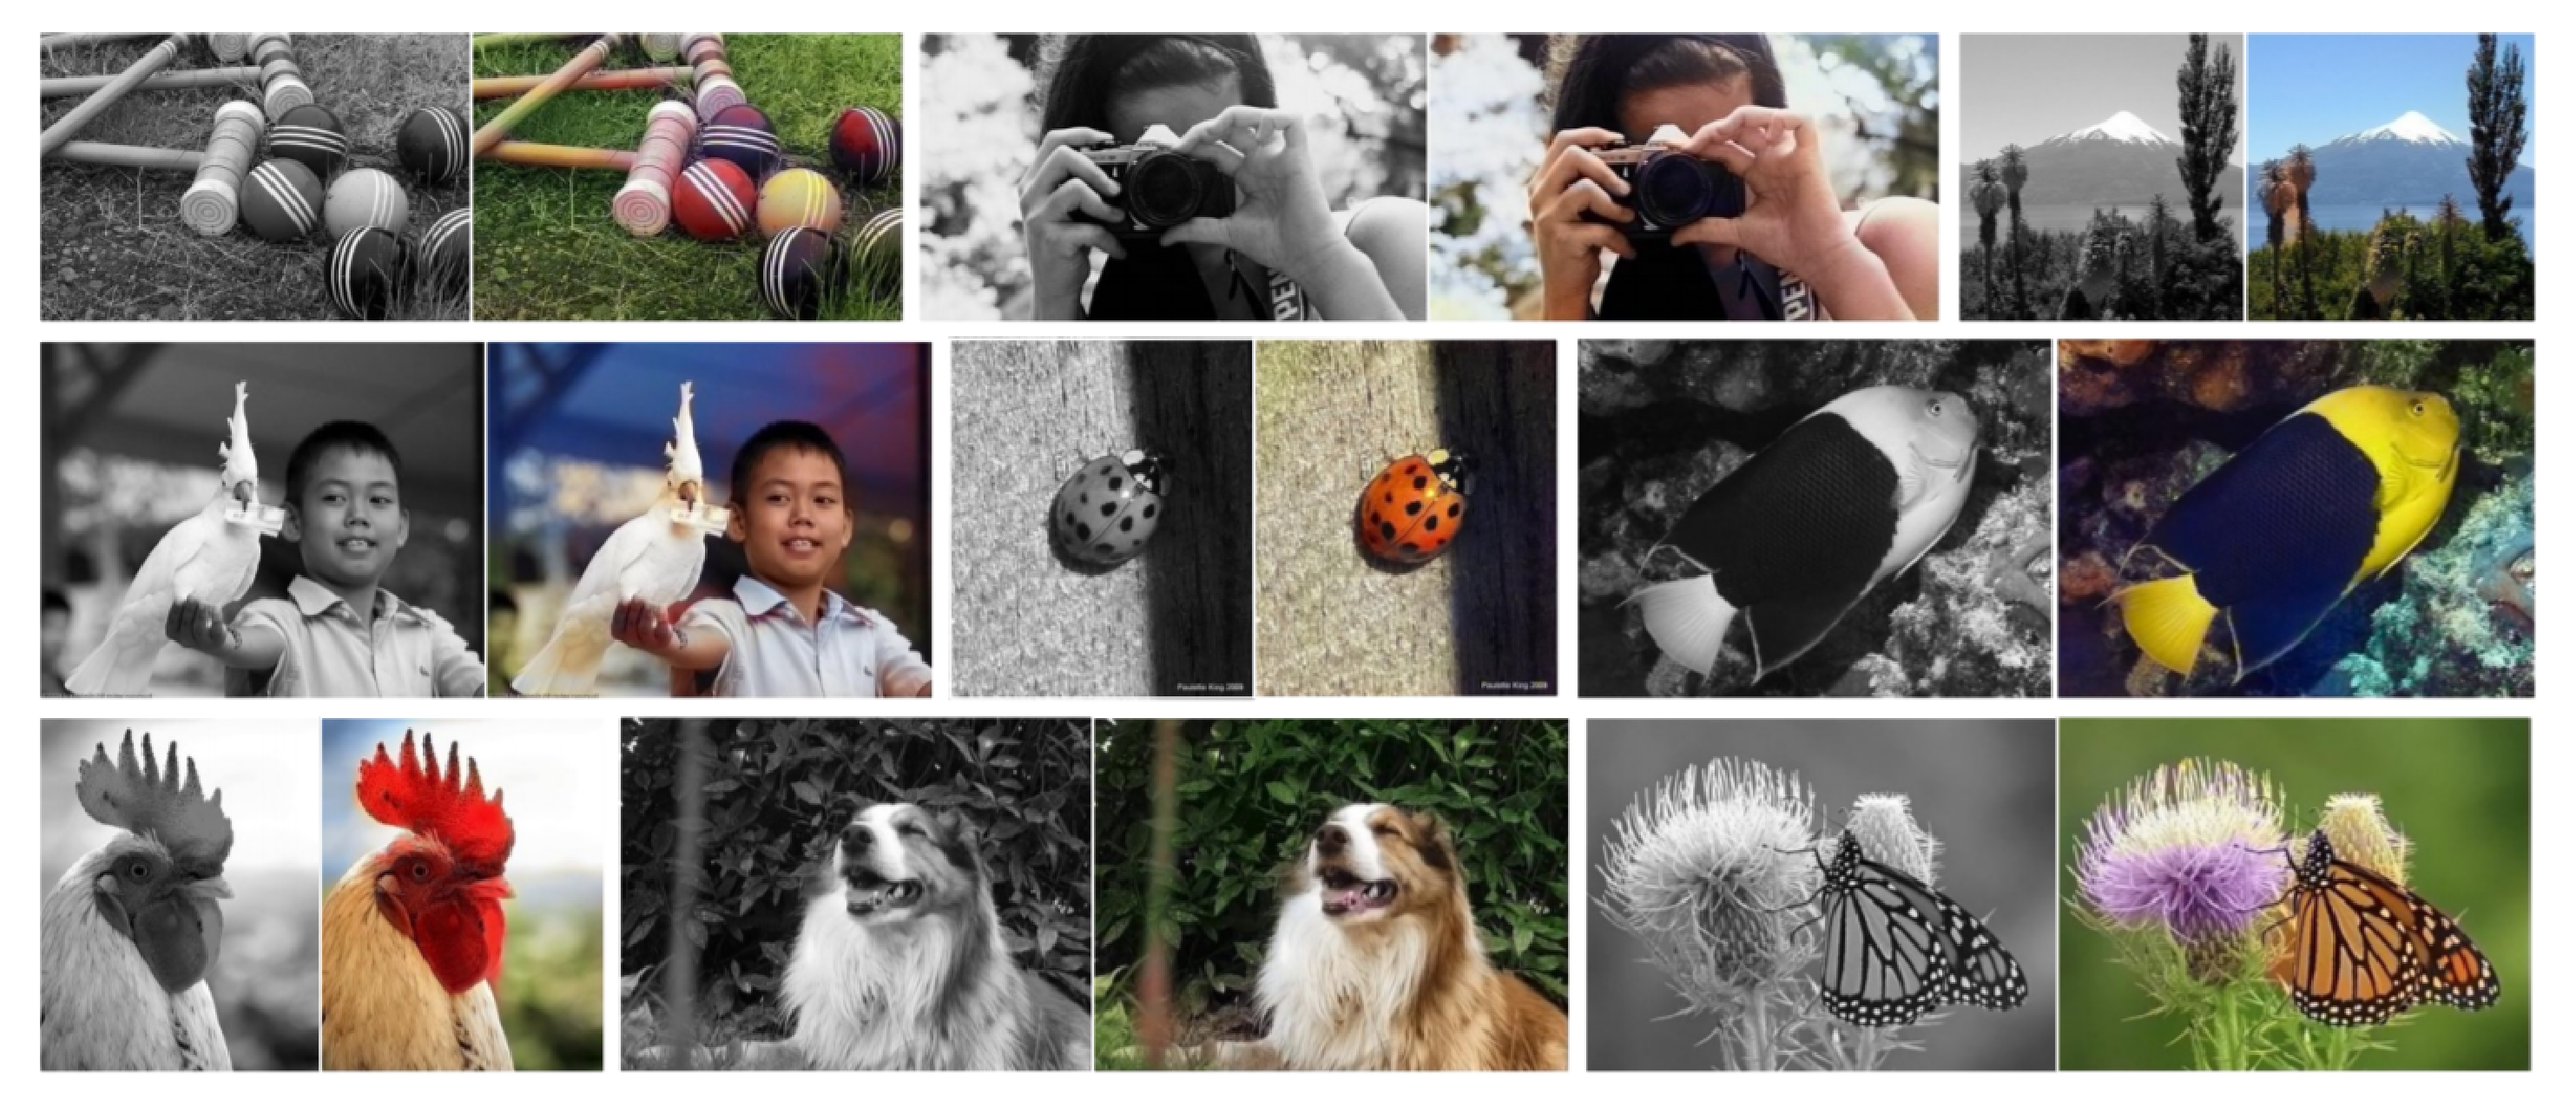
\includegraphics[width=0.7\paperwidth]{appendixF1}
  \caption*{图~1\quad 输入的灰度图像和通过我们的算法输出的彩色结果的样例。这些是选出来的非常好的结果。如果想看所有的结果或者尝试我们的模型和代码,请访问\url{http://richzhang.github.io/colorization/}}
  \label{tab:badfigure1}
\end{figure}

给定亮度通道L,我们的系统在CIE Lab颜色空间预测图像对应的a和b颜色通道。为了解决这个问题,我们利用了大数据。 预测颜色有一点很好的属性就是训练数据是免费可得的:任何彩色照片都可以用作训练样本,简单的通过将图像的L通道作为输入以及其ab通道作为标定结果。 有人也注意到训练数据的易得性,并且之前的工作已经训练了卷积神经网络(CNN)用来预测大数据集上的颜色[1,2]。 然而,之前工作的结果倾向于看起来不饱和。 一个解释是[1,2]他们使用了鼓励保守预测的损失函数。 这些偏差来源于标准回归问题,而标准回归问题的目标是在预测结果和真实值之间最小化欧氏距离。

相反我们使用了针对着色问题的损失函数。 正如[3]中指出的,颜色预测本质上是多模式的 - 许多物体可以有好几种可能的合理着色。 例如,苹果通常是红色,绿色或黄色的,但不可能是蓝色或橙色。为了给这个多模态问题适当地建模 ,我们对每个像素预测了可能颜色的分布。此外,为了强调稀有的颜色,在训练时我们重新调整了损失。这鼓励我们的模型在训练集上探索大量数据的全面多样性。 最后,我们通过在颜色分布上取退火平均值的方法产生最终的着色结果。 最终的结果相比之前的方法就有更加生动的色彩并且视觉上更逼真。

评估合成的图像是一个众所周知的难题[4]。 因为我们的终极目标是使结果令观察者信服,我们引入了一种新颖的评估着色结果的方法——直接测试它们的现实真实感。 我们建立了一个“色彩图灵测试”,在测试中展示给参与者一张真实图像和这张图像的机器着色版本,要求他们识别出假的图像。在这个相当困难的标准中,我们能够在32\%实例(两张都是真实照片的话概率将是50\%)中欺骗参与者,显著高于以前的工作[2]。 这个测试表明,在许多情况下,我们的算法都产生近似逼真的结果(参见图1的经过挑选的我们算法的成功例子)。 我们还展示了这个系统对于下游任务是足够真实以至于有用的,特别是使用现成的VGG网络的物体识别[5]。

我们另外探讨了着色作为一种自监督学习的形式,这种学习中原始数据被用作自己的监督来源。这种特征学习表示的想法至少可以追溯到自动编码器[6]。 最近有更多的工作通过数据估算探讨了特征学习,在其中完整数据的一部分被拿出来做预测(例如,[7,8,9,10,11,12,13])。我们的方法也是这种方式,并且可以被称为交叉信道编码器。我们测试了自己的模型在通用任务中的表现,与之前的[14,8,15,10]和同时[16]自我监督算法相比,发现我们的方法表现出色,在几个测试中都能达到最好的表现。

我们在本文中的贡献体现在两个方面。 首先,我们在自动图像着色的图形学问题取得了进展,通过(a)设计适当的目标函数来处理多模态的不确定性着色问题并且能够抓取各种各样的颜色,(b)引入一个用于测试着色算法的新框架,还可能适用于其他图像合成任务,以及(c)在这个任务上通过百万照片的训练设立了新的高水准。 其次,我们在着色任务中提出了一种有竞争力且直接的自监督学习方法,在几个基准上实现了最先进的结果。

$\textbf{以前的着色工作}$ 着色算法的主要区别在于他们对于建模灰度和颜色之间关系时获得和处理数据的方式。 非参数方法,给定输入的灰度图像,首先定义一个或多个彩色参考图像(由用户提供或自动检索)用作源数据。 然后,按照图像类比框架[17],颜色从参考图像的类比区域转移到输入图像[18,19,20,21]。另一方面,参数方法,在训练时从彩色图像的大数据集学习预测函数,将问题作为连续色彩空间的回归问题[22,1,2]或量化色值的分类问题[3]。 我们的方法也学习分类颜色,但是使用了更大的模型,训练了更多的数据,并且在损失函数和映射到一个连续结果上有一些创新。

$\textbf{同时的着色工作}$ 与我们的论文同时的,Larsson等人 [23]和Iizuka等人 [24]已经开发出类似的系统,他们也利用了大规模数据和CNN。这些方法区别在于CNN的结构以及损失函数。我们使用了分类损失,重新平衡稀有类,而Larsson 等人使用未重新平衡的分类损失,而Iizuka等人用了回归损失。在3.1节中,我们在我们的网络结构上比较了每种类型的损失函数的效果。 CNN结构也有所不同:Larsson等人在VGG[5]上使用了多列网络[25] ,Iizuka等人使用双流结构,融合全局和局部特性,而我们使用单流,VGG风格的网络并且添加了深度和扩张的卷积层[26,27]。此外,我们和Larsson等人是在ImageNet上训练我们的模型[28],Iizuka等人在Places训练他们的模型[29]。在3.1节,我们提供了与Larsson等人的量化比较,并且鼓励感兴趣的读者调研两个同时的论文。

\begin{figure}[h]
  \centering
  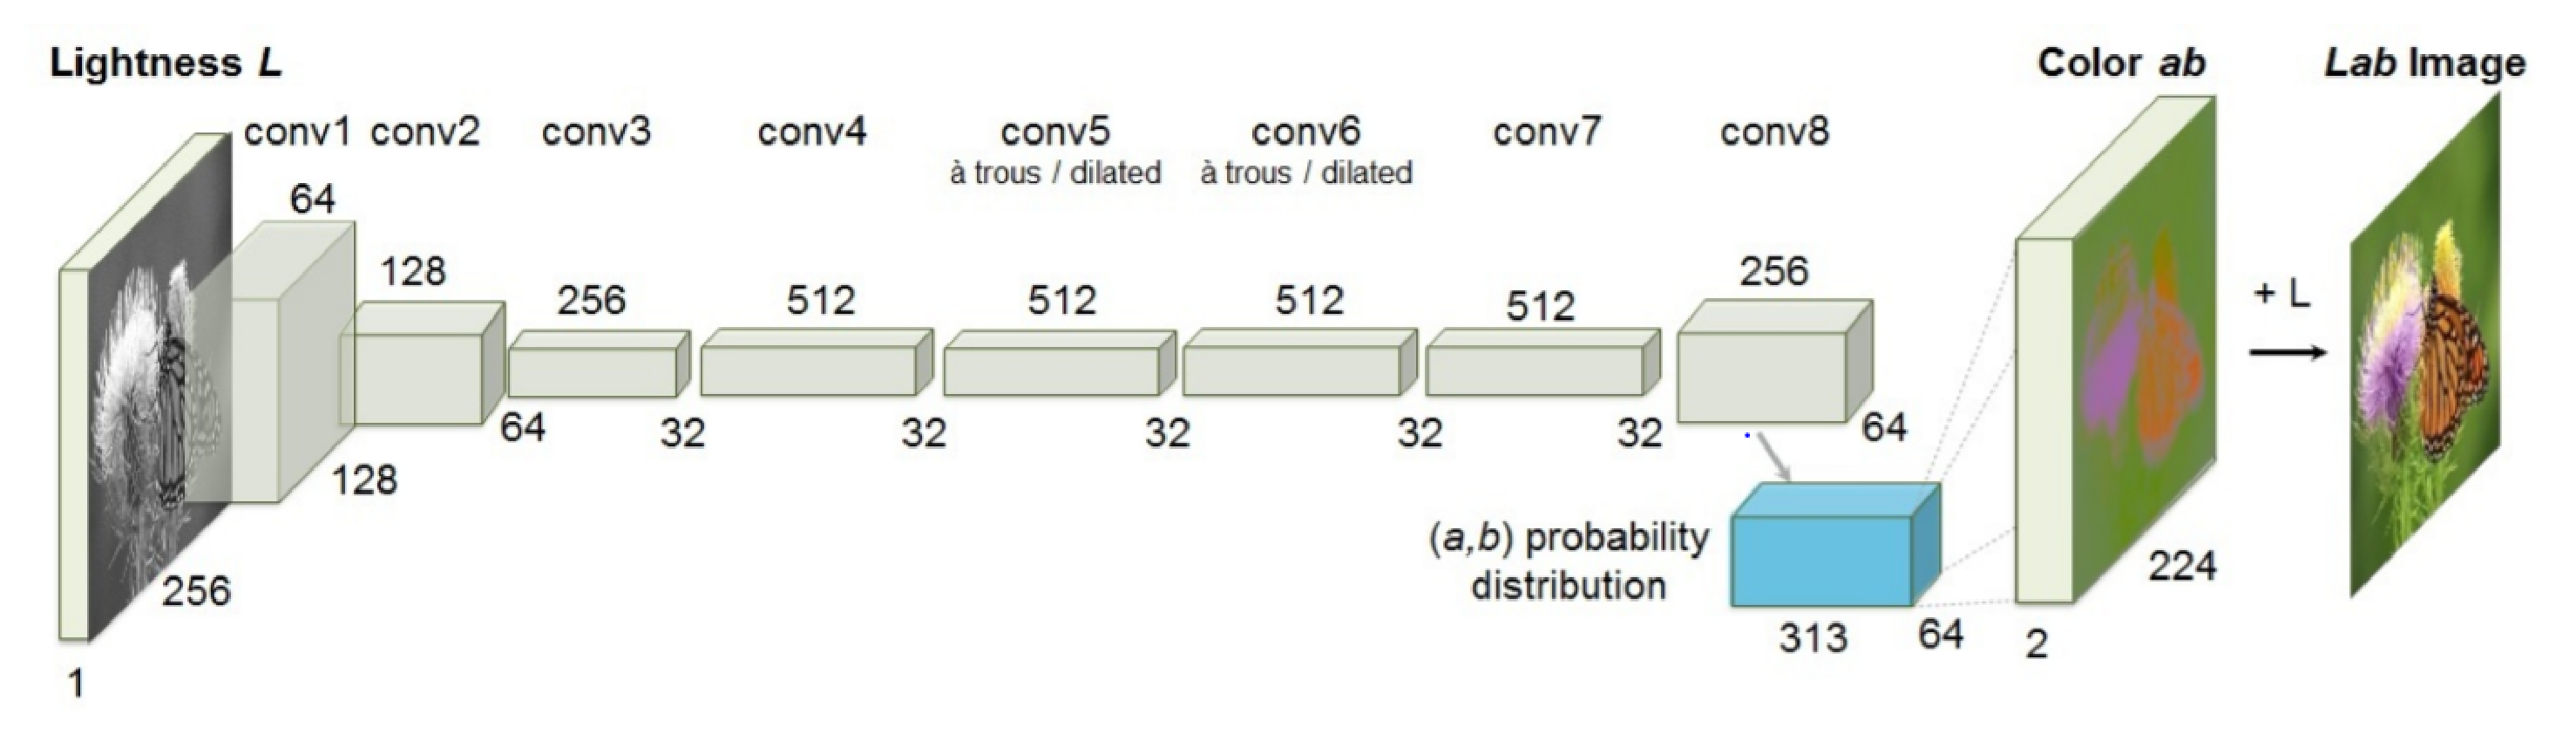
\includegraphics[width=0.7\paperwidth]{appendixF2}
  \caption*{图~2\quad 我们的网络结构。每个conv层代表2到3个重复conv和ReLU层的集合,跟着一个BatchNorm[30]层。这个网络没有池化层。解决方案中所有的改变都来源于在卷积块之间的空间下采样和上采样。}
  \label{tab:badfigure2}
\end{figure}

\section{方法}
我们训练了一个CNN从灰度输入映射到量化颜色值输出的分布,使用图2所示的结构。结构细节在我们的项目网页的补充材料中给出了描述,且该模型是公开可用的。 接下来,我们专注于目标函数的设计,以及我们的用于从预测的颜色分布中推断点颜色的技术。

\subsection{目标函数}
给定输入的亮度通道$X \in \mathbb{R}^{H \times W \times 1}$,我们的目标是学习一个到两个相关联的彩色通道$Y \in \mathbb{R}^{H \times W \times 2}$的映射$\hat{Y} = \mathcal{F}(X)$,在这里$H, W$是图像的大小。(我们给预测结果加了一个$\hat{.}$标志而真实结果没有)我们在CIE Lab颜色空间上进行的这个任务。由于这个空间上的距离建模了视觉上的距离,在[1,2]中使用的一个自然的目标函数,就是在预测结果的颜色和真实结果颜色之间的欧式距离$L_2(.,.)$:

\begin{equation}\tag*{(1)}
L_2(\hat{Y}, Y) = \frac{1}{2}\sum_{h,w}\|Y_{h,w} - \hat{Y}_{h,w}\|_{2}^{2}
\end{equation}

但是,这个损失在面对着色问题的固有模糊性和多模态时不够鲁棒。如果一个物体可以在取一系列的不同ab值,欧式距离损失的最优解就会是这些值的平均值。在颜色预测中,这种平均的效果倾向于灰色和不饱和的结果。另外,如果合理着色的集合是非凸的,那么平均结果可能会落在合理区域外,从而给出不合理的结果。

\begin{figure}[h]
  \centering
  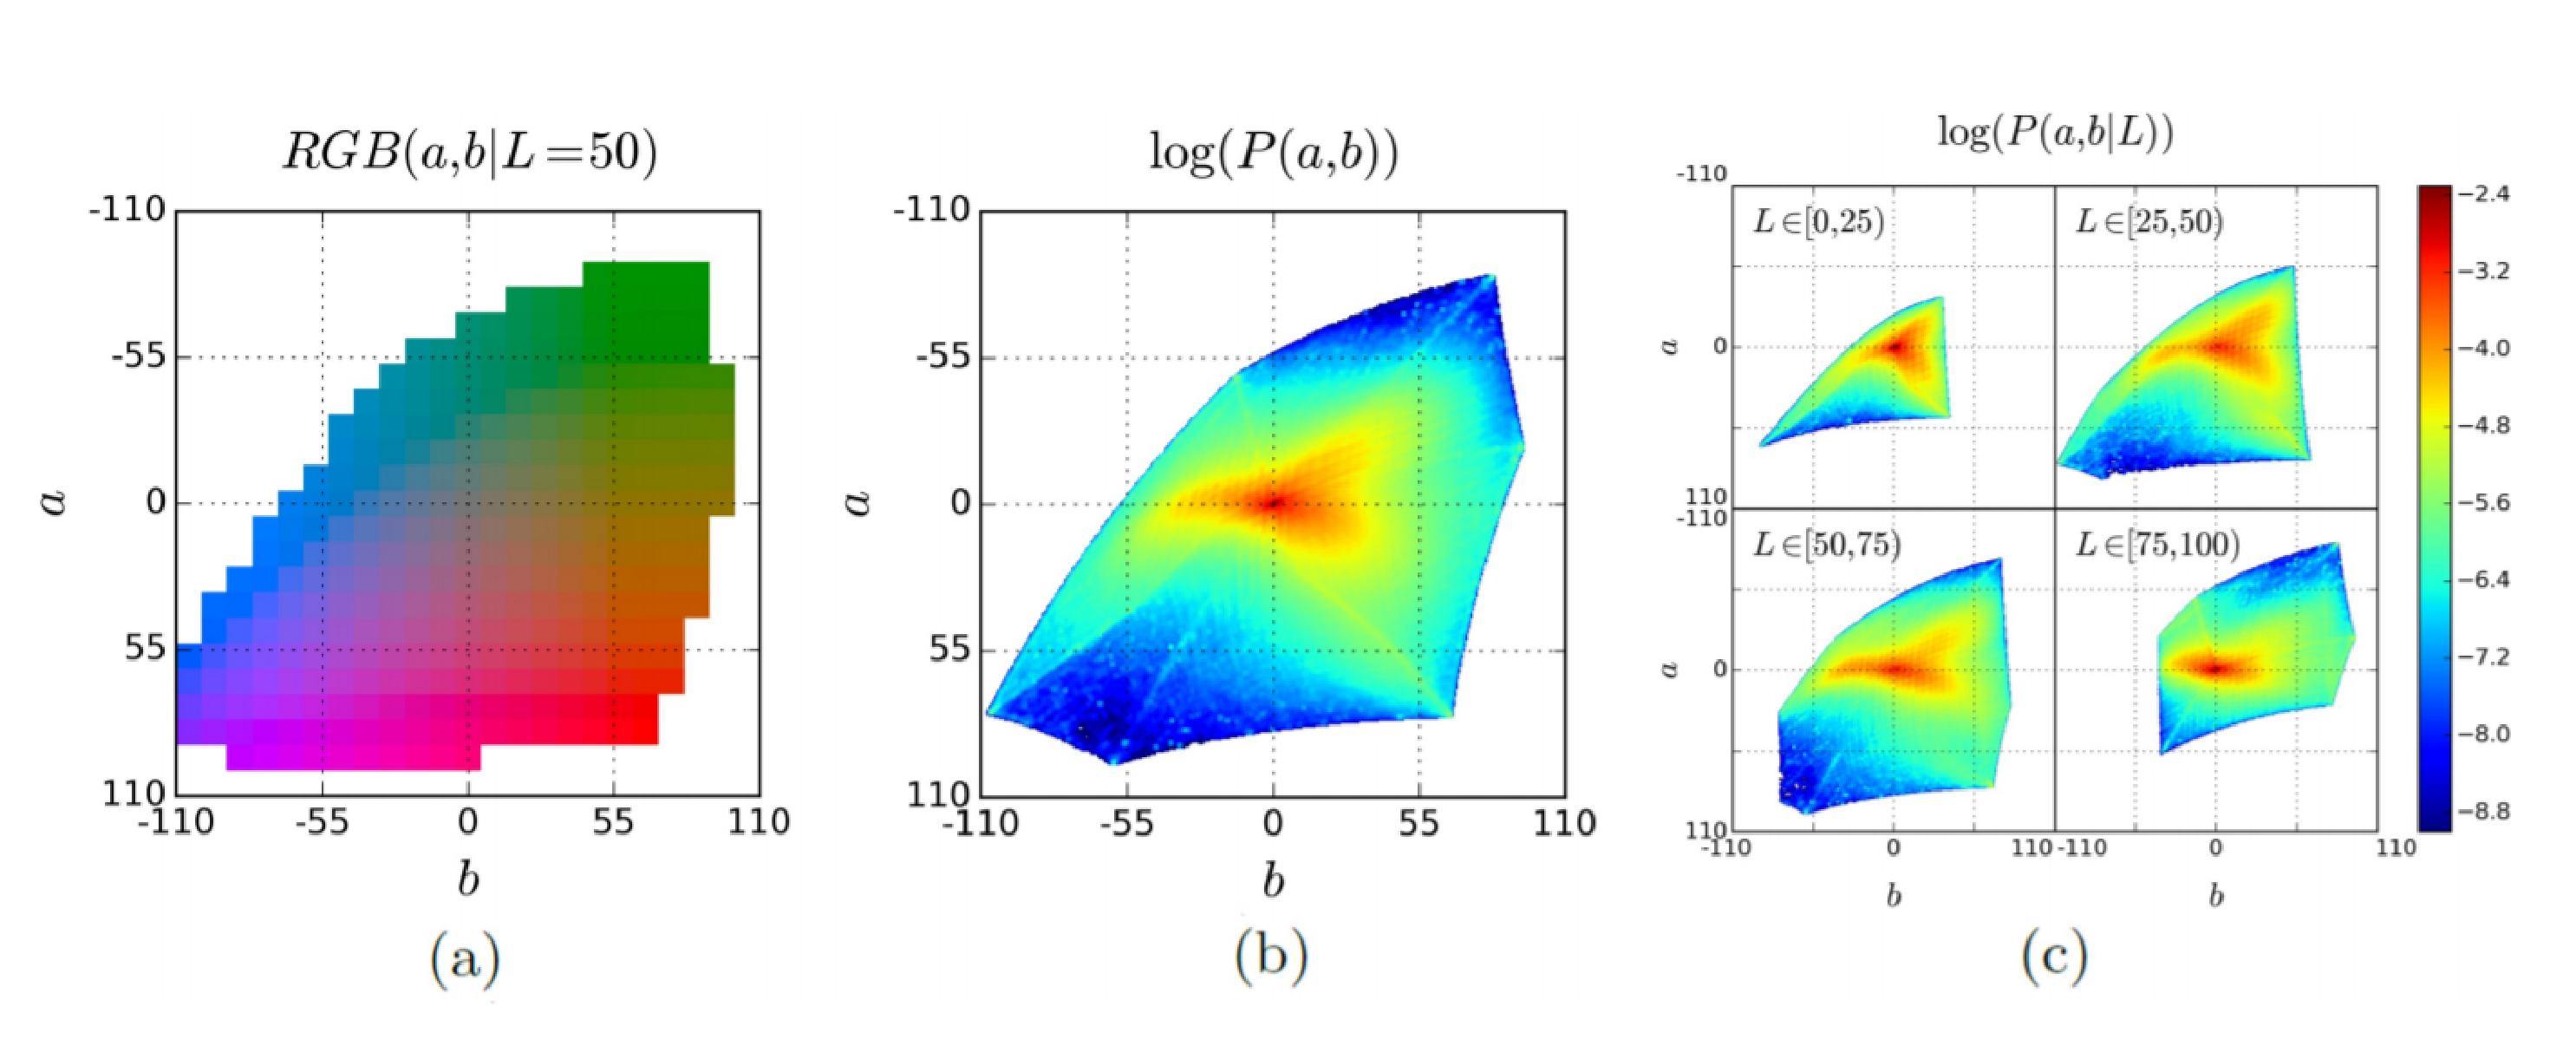
\includegraphics[width=0.7\paperwidth]{appendixF3}
  \caption*{图~3\quad (a)用大小为10的方格量化后的ab色彩空间。色域中总共包含313个ab色彩对。(b)ab颜色的经验分布,在log尺度下显示(c)在给定L值条件下的ab颜色经验分布,在log尺度下显示。}
  \label{tab:badfigure3}
\end{figure}

相反,我们把这个问题当成一个多模态的分类问题。我们将ab色彩空间量化为方格大小为10的桶并且保留了在色域的$Q = 313$个值,如图3(a)所示。对于给定的输入$Xs$,我们学习了一个到可能颜色$\hat{Z} \in [0,1]^{H \times W \times Q}$概率分布的映射$\hat{Z} = \mathcal{G}(X)$,在这里$Q$是量化后ab值的数量。

为了比较预测的结果$\hat{Z}$与真实结果,我们定义了一个将真实颜色$Y$转换到向量$Z$的函数$Z = \mathcal{H}^{-1}_{gt}(Y)$,使用的是软编码方案。我们然后使用了多模态的交叉熵损失$L_{cl}(.,.)$,定义为

\begin{equation}\tag*{(2)}
L_{cl}(\hat{Z}, Z) = -\sum_{h,w}v(Z_{h,w})\sum_{q}Z_{h,w,q} \log(\hat{Z}_{h,w,q})
\end{equation}

在这里$v(.)$是一个权重项,可以用来重新平衡稀有的颜色类别的损失,在下面的2.2节定义。最后我们用映射函数$\hat{Y}=\mathcal{H}(\hat{Z})$将概率分布$\hat{Z}$映射到颜色值$\hat{Y}$,这会在2.3节讨论。

\subsection{类别重新平衡}

由于背景的表现例如云朵,人行道,尘土和围墙,自然图片中的ab值的分布严重倾向于很低。图3(b)显示了在ab空间像素的经验分布,数据来源于ImageNet的130万张训练图片[28]。观察到自然图片中的不饱和像素的数量比饱和像素的数量高出了几个数量级。如果不考虑到这一点,损失函数就会被不饱和ab值占据。我们通过在训练时基于像素颜色的稀有度重新加权了每个像素的损失来针对这个问题。这渐近地等同于典型的对训练空间重新采样的方法[32]。每个像素被一个因素$w \in \mathbb{R}^Q$衡量,基于它最近的ab颜色桶。

\begin{equation}\tag*{(3)}
v(Z_{h,w}) = w_{q^*}, \text{where } q^* = \text{arg } \max\limits_{q} Z_{h,w,q}
\end{equation}

\begin{equation}\tag*{(4)}
w \propto ((1-\lambda)\tilde{p}+\frac{\lambda}{Q})^{-1},\text{ } \mathbb{E}[w] = \sum_{q}\tilde{p}_{q}w_q = 1
\end{equation}

为了获得平滑的经验颜色分布$\tilde{p} \in \Delta^Q$,我们从整个ImageNet训练集统计了经验的量化的ab空间的概率分布$p \in \Delta^Q$并且用一个高斯核$\text{G}_{\sigma}$将分布做了平滑处理。然后我们将这个分布用一个权值$\lambda \in [0,1]$与一个标准分布混合,采取倒数并且归一化所以权重因子的期望是1。我们发现$\lambda = \frac{1}{2}$和$\sigma = 5$效果很好。在3.1节里我们将这个结果与没有做类别重新平衡的结果进行了对照。

\subsection{从类别概率到点估计}

最终,我们定义了$\mathcal{H}$,是从预测的分布$\hat{Z}$到ab颜色空间$\hat{Y}$的映射。一种选择是对于每个像素取其预测分布的最大值,正如图4中最右一列所示的两个例子。这提供了一种富有活力的着色结果但是有时会造成空间不连续的结果,例如大巴上的红色斑点。从另一方面,取预测分布的平均值会造成空间上连续但是不饱和的结果(图4中的最左列),呈现一种不自然的棕褐色调。这是不令人惊讶的,因为在做分类处理之后取平均值与使用欧式距离作为损失函数的回归架构有一样的问题。为了在以上两方面都取得最好的结果,我们通过调整参数T来内插softmax分布,并且取了结果的平均值。我们的灵感来源于模拟退火技术[33],因此称这个操作为取分布的退火平均值。

\begin{equation}\tag*{(5)}
\mathcal{H}(Z_{h,w}) = \mathbb{E}[f_T(Z_{h,w})], \text{ } f_T(z) = \frac{\exp(\log(z)/T)}{\Sigma_q\exp(\log(Z_q)/T)}
\end{equation}

设T=1使得这个分布没有改变,降低温度使得分布更突出一些极值点,而当$T \rightarrow 0$会得到分布的单热点编码。我们发现当温度T=0.38,如图4的中间一列所示,能捕捉到活力性同时也维持空间连续性。

我们最终的系统$\mathcal{F}$是CNN $\mathcal{G}$与退火平均值操作$\mathcal{H}$的结合体,前者对所有像素生成了概率分布,后者生成最终的着色结果这个系统不能完全端到端的训练,但是记住一点就是这个映射$\mathcal{H}$对每个像素独立操作,只包含一个参数,并且可以实现为CNN前向传递的一部分。

\begin{figure}[h]
  \centering
  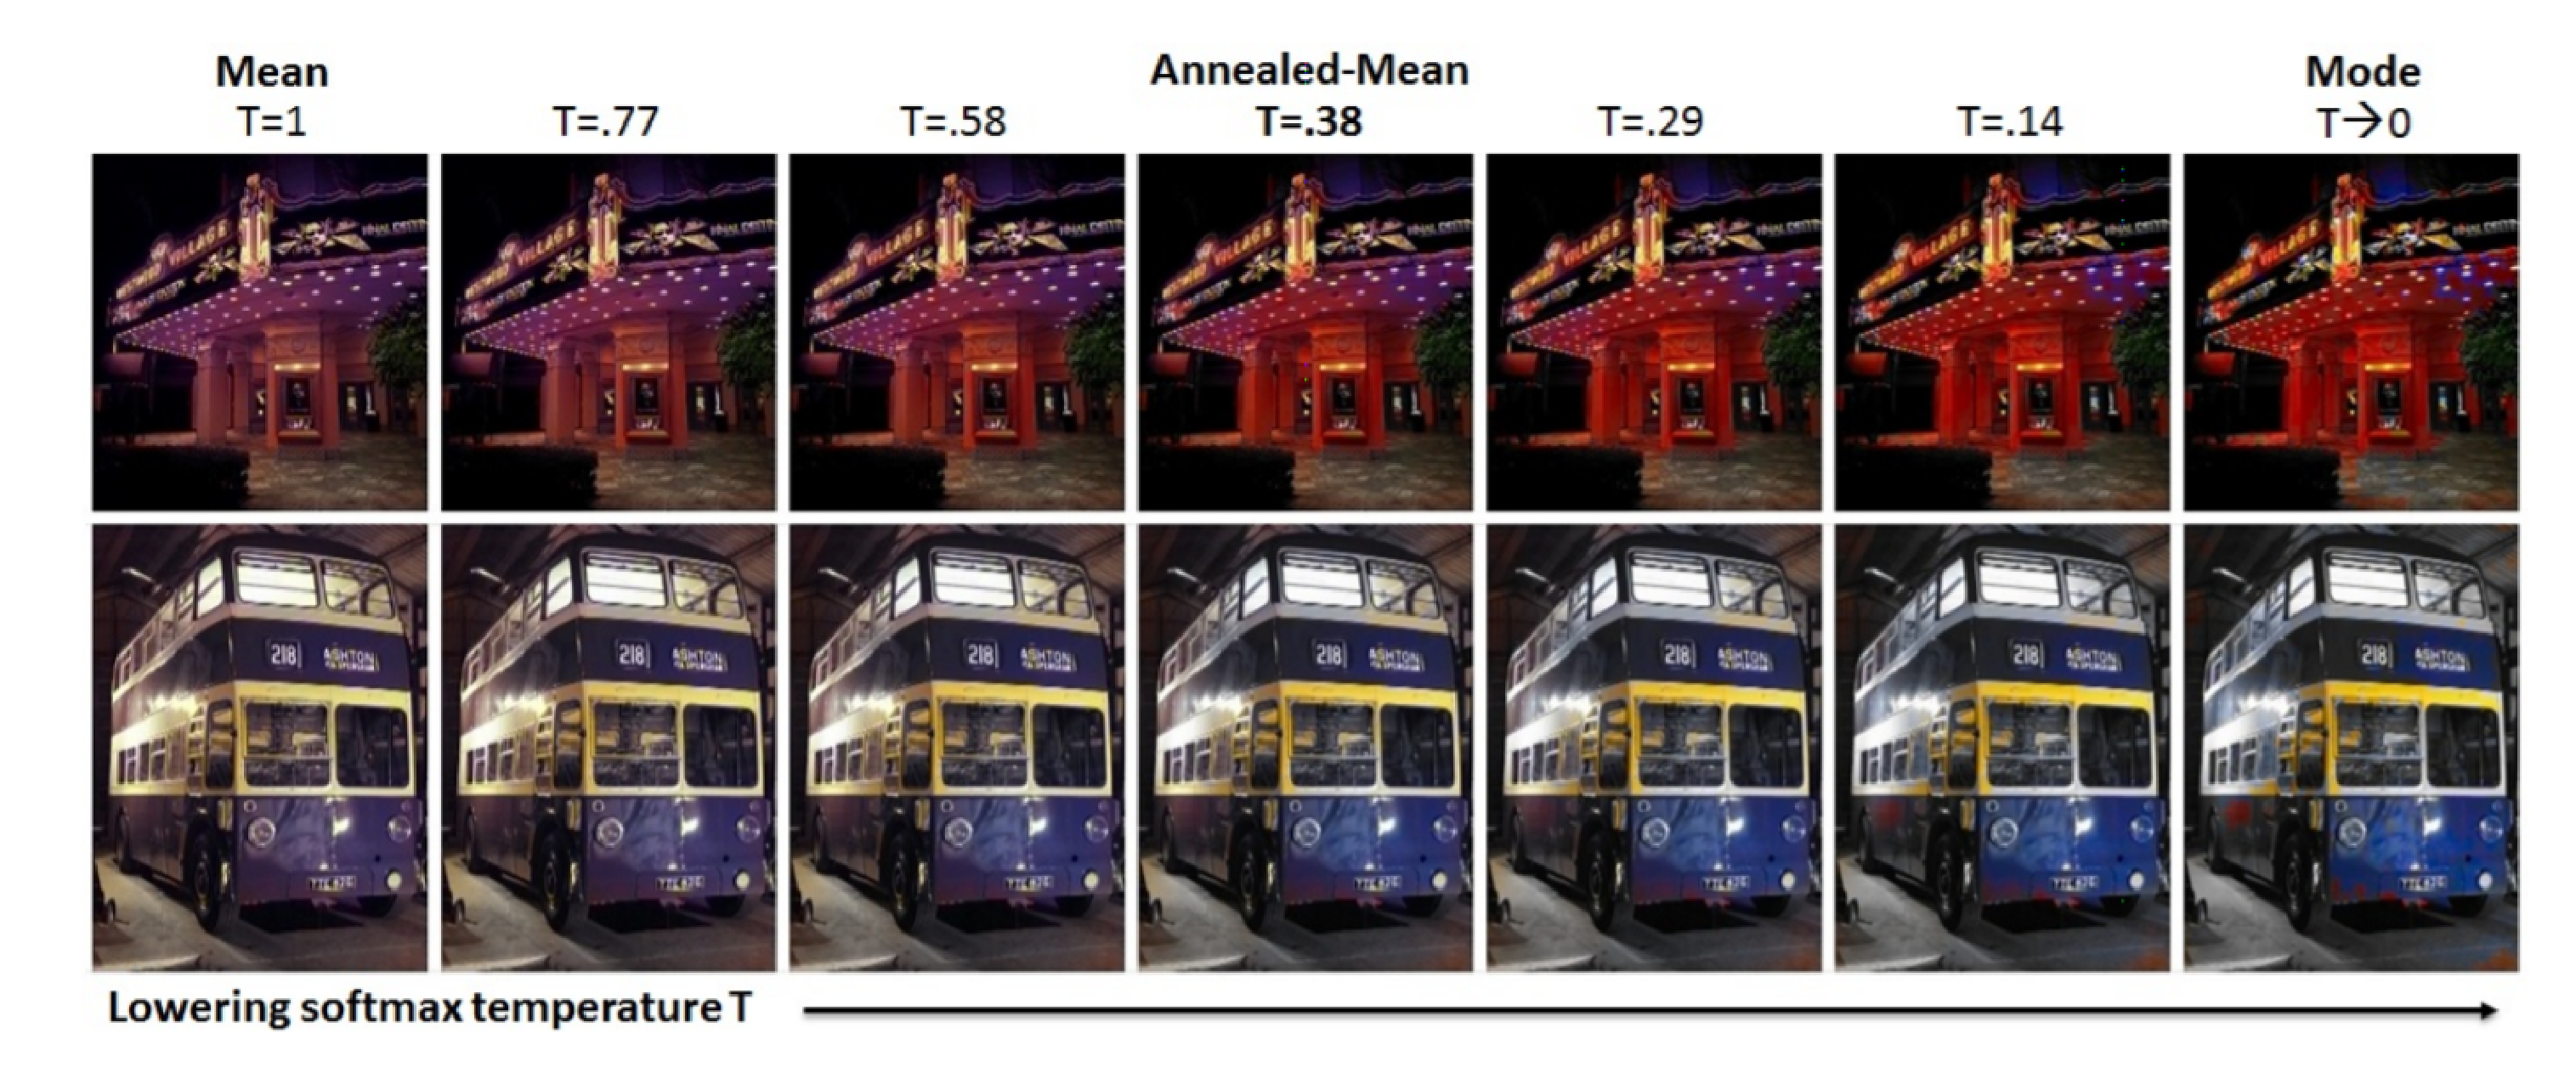
\includegraphics[width=0.7\paperwidth]{appendixF4}
  \caption*{图~4\quad 温度参数T对退火平均值输出的效果(公式5)最左边的图像是预测颜色的平均值,最右边的是取最可能的颜色值。在我们的系统中T=0.38}
  \label{tab:badfigure4}
\end{figure}

\section{实验}

在3.1节,我们在图像层面评估了我们的算法,评估了我们着色结果的视觉真实感,也使用了其他准确度评估方式。我们将自己完整的算法与几个变体以及最近[2]和同时的工作[3]做了对比。在3.2节,我们测试了着色作为一种自监督学习的方法。最后,在10.1节,我们展示了给真实老黑白照片着色的定性结果。

\begin{figure}[!htb]
  \centering
  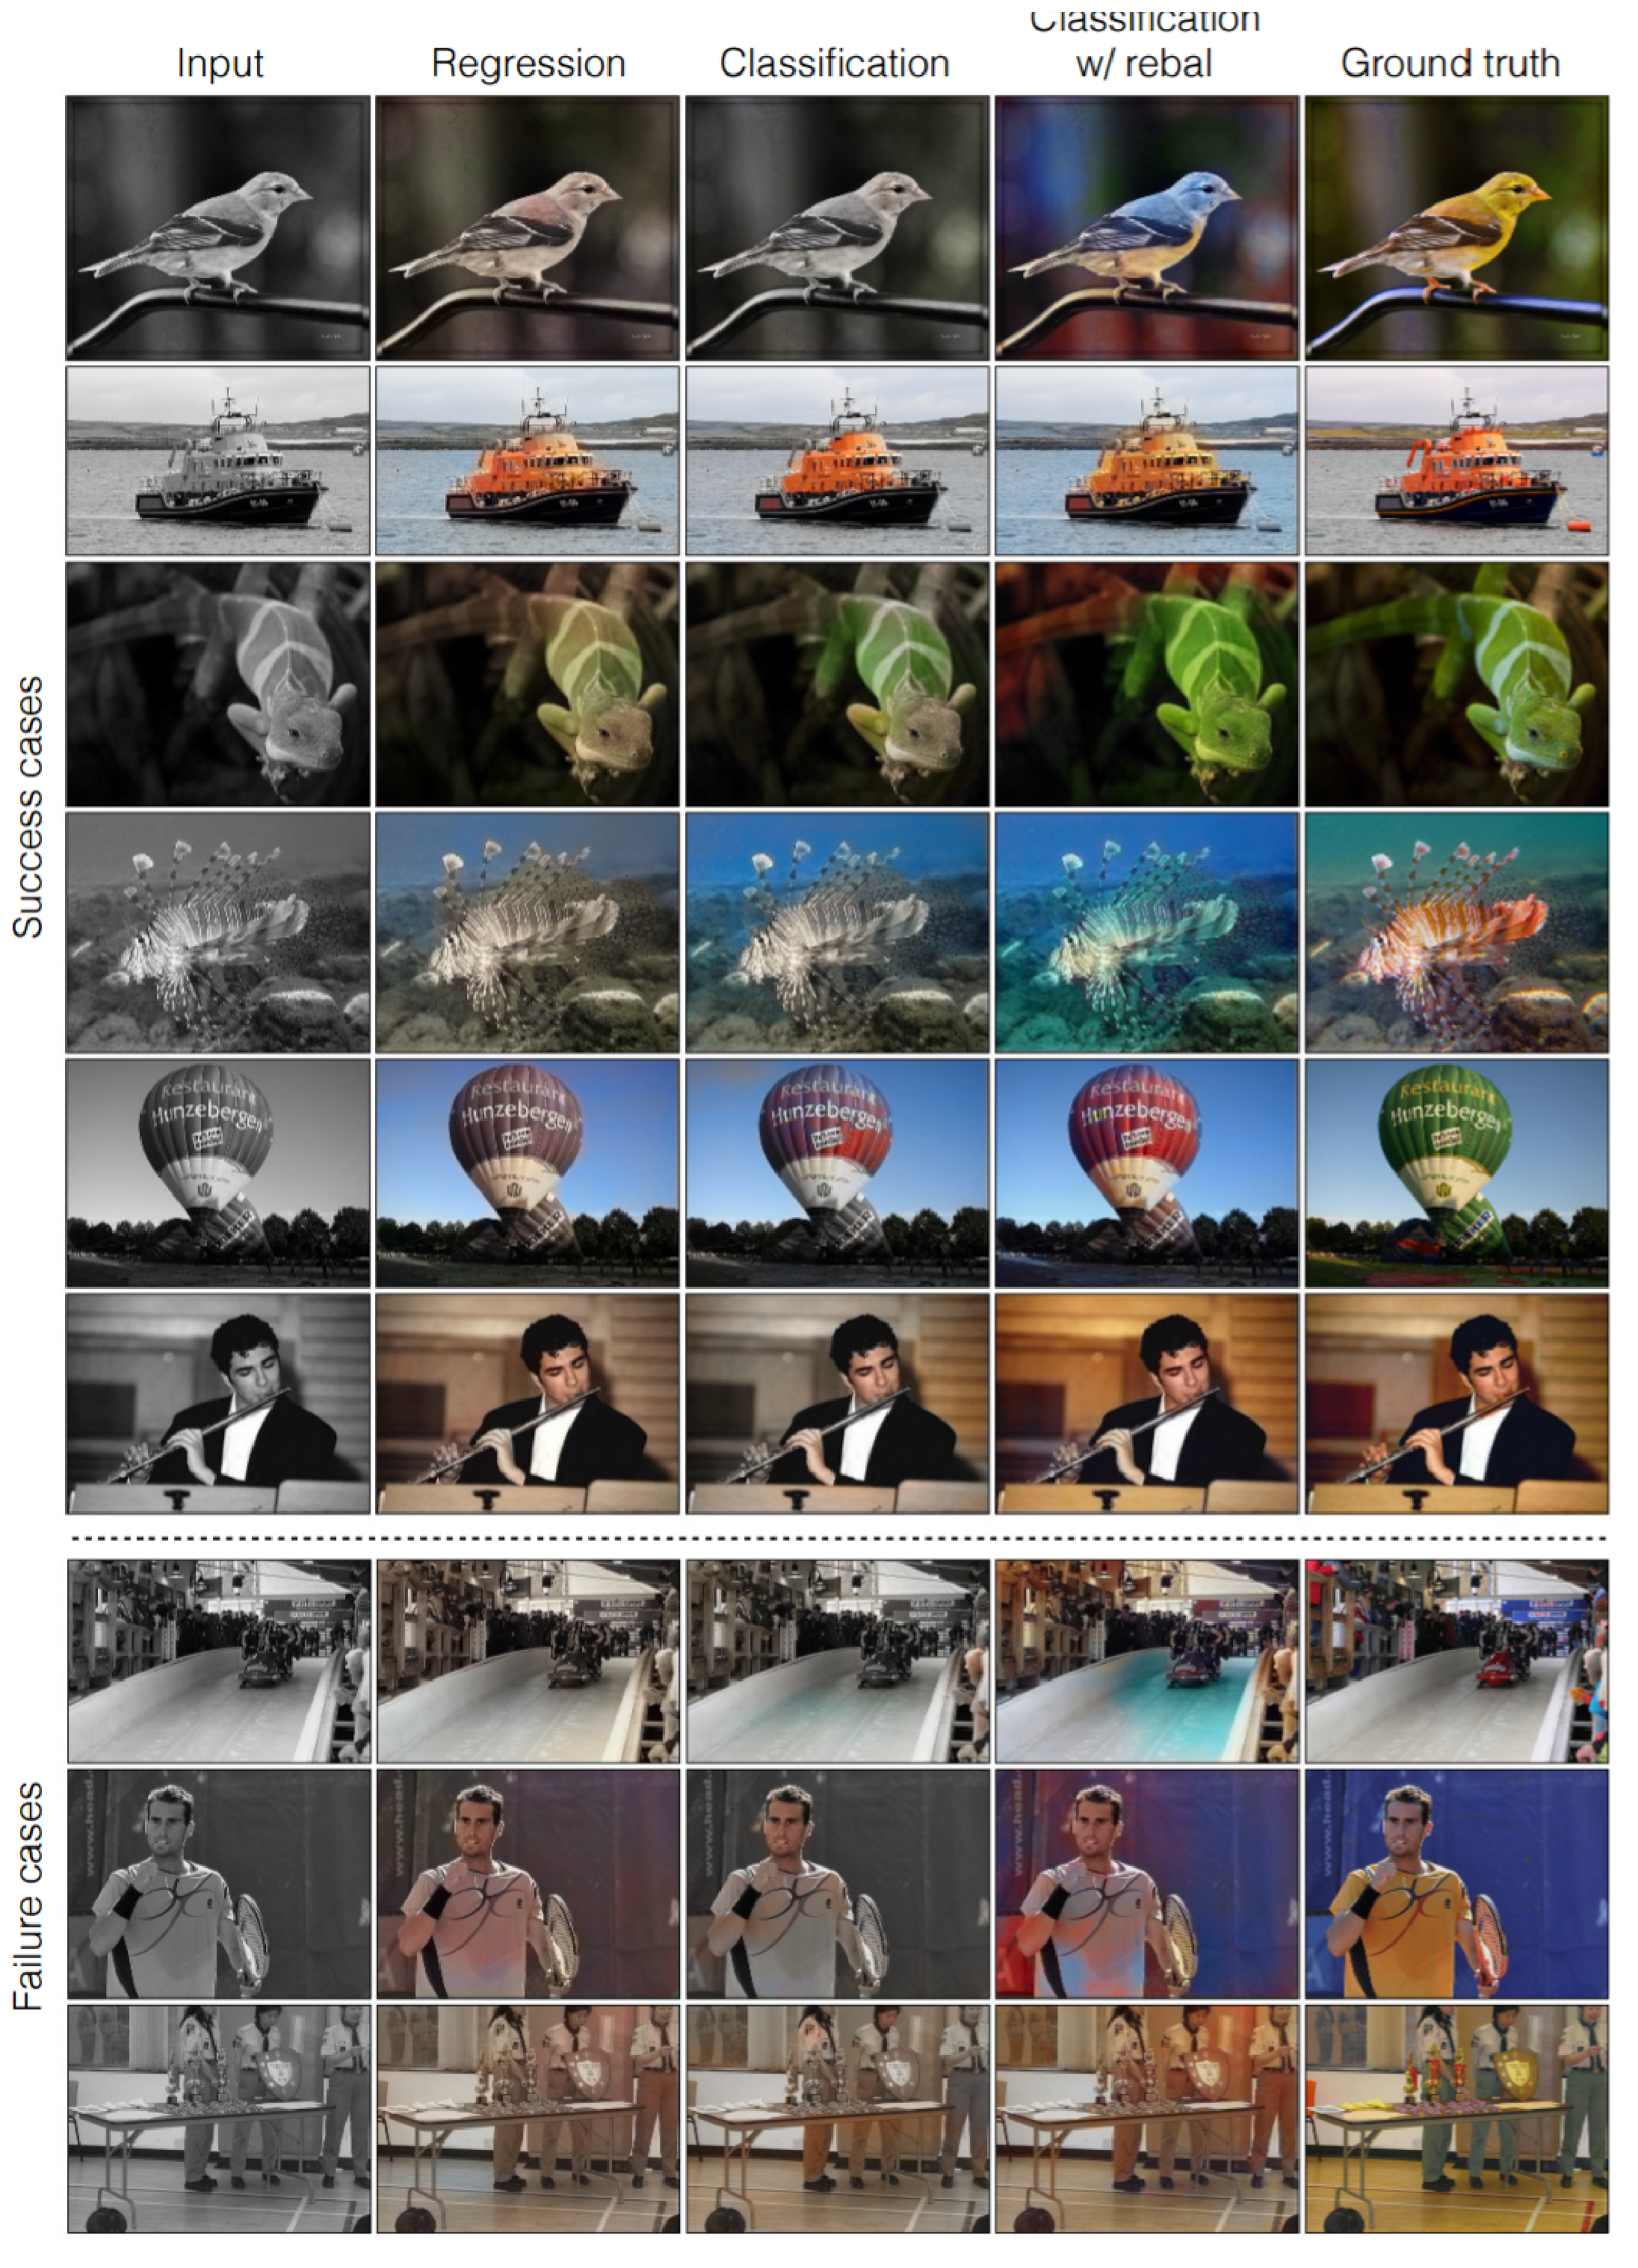
\includegraphics[width=0.6\paperwidth]{appendixF5}
  \caption*{图~5\quad 来自ImageNet测试集的结果。我们的分类损失和重新平衡比回归损或者没有重新平衡的分类损失制造了更准确和更有活力的结果。在点线上方是成功的着色,常见的失败案例在下方。其中包含不能抓取大范围连续性的失败,红色和蓝色之间的冲突,和室内场景的棕褐色调。访问\url{http://richzhang.github.io/colorization/}查看完整的结果。}
  \label{tab:badfigure5}
\end{figure}

\begin{figure}[h]
  \centering
  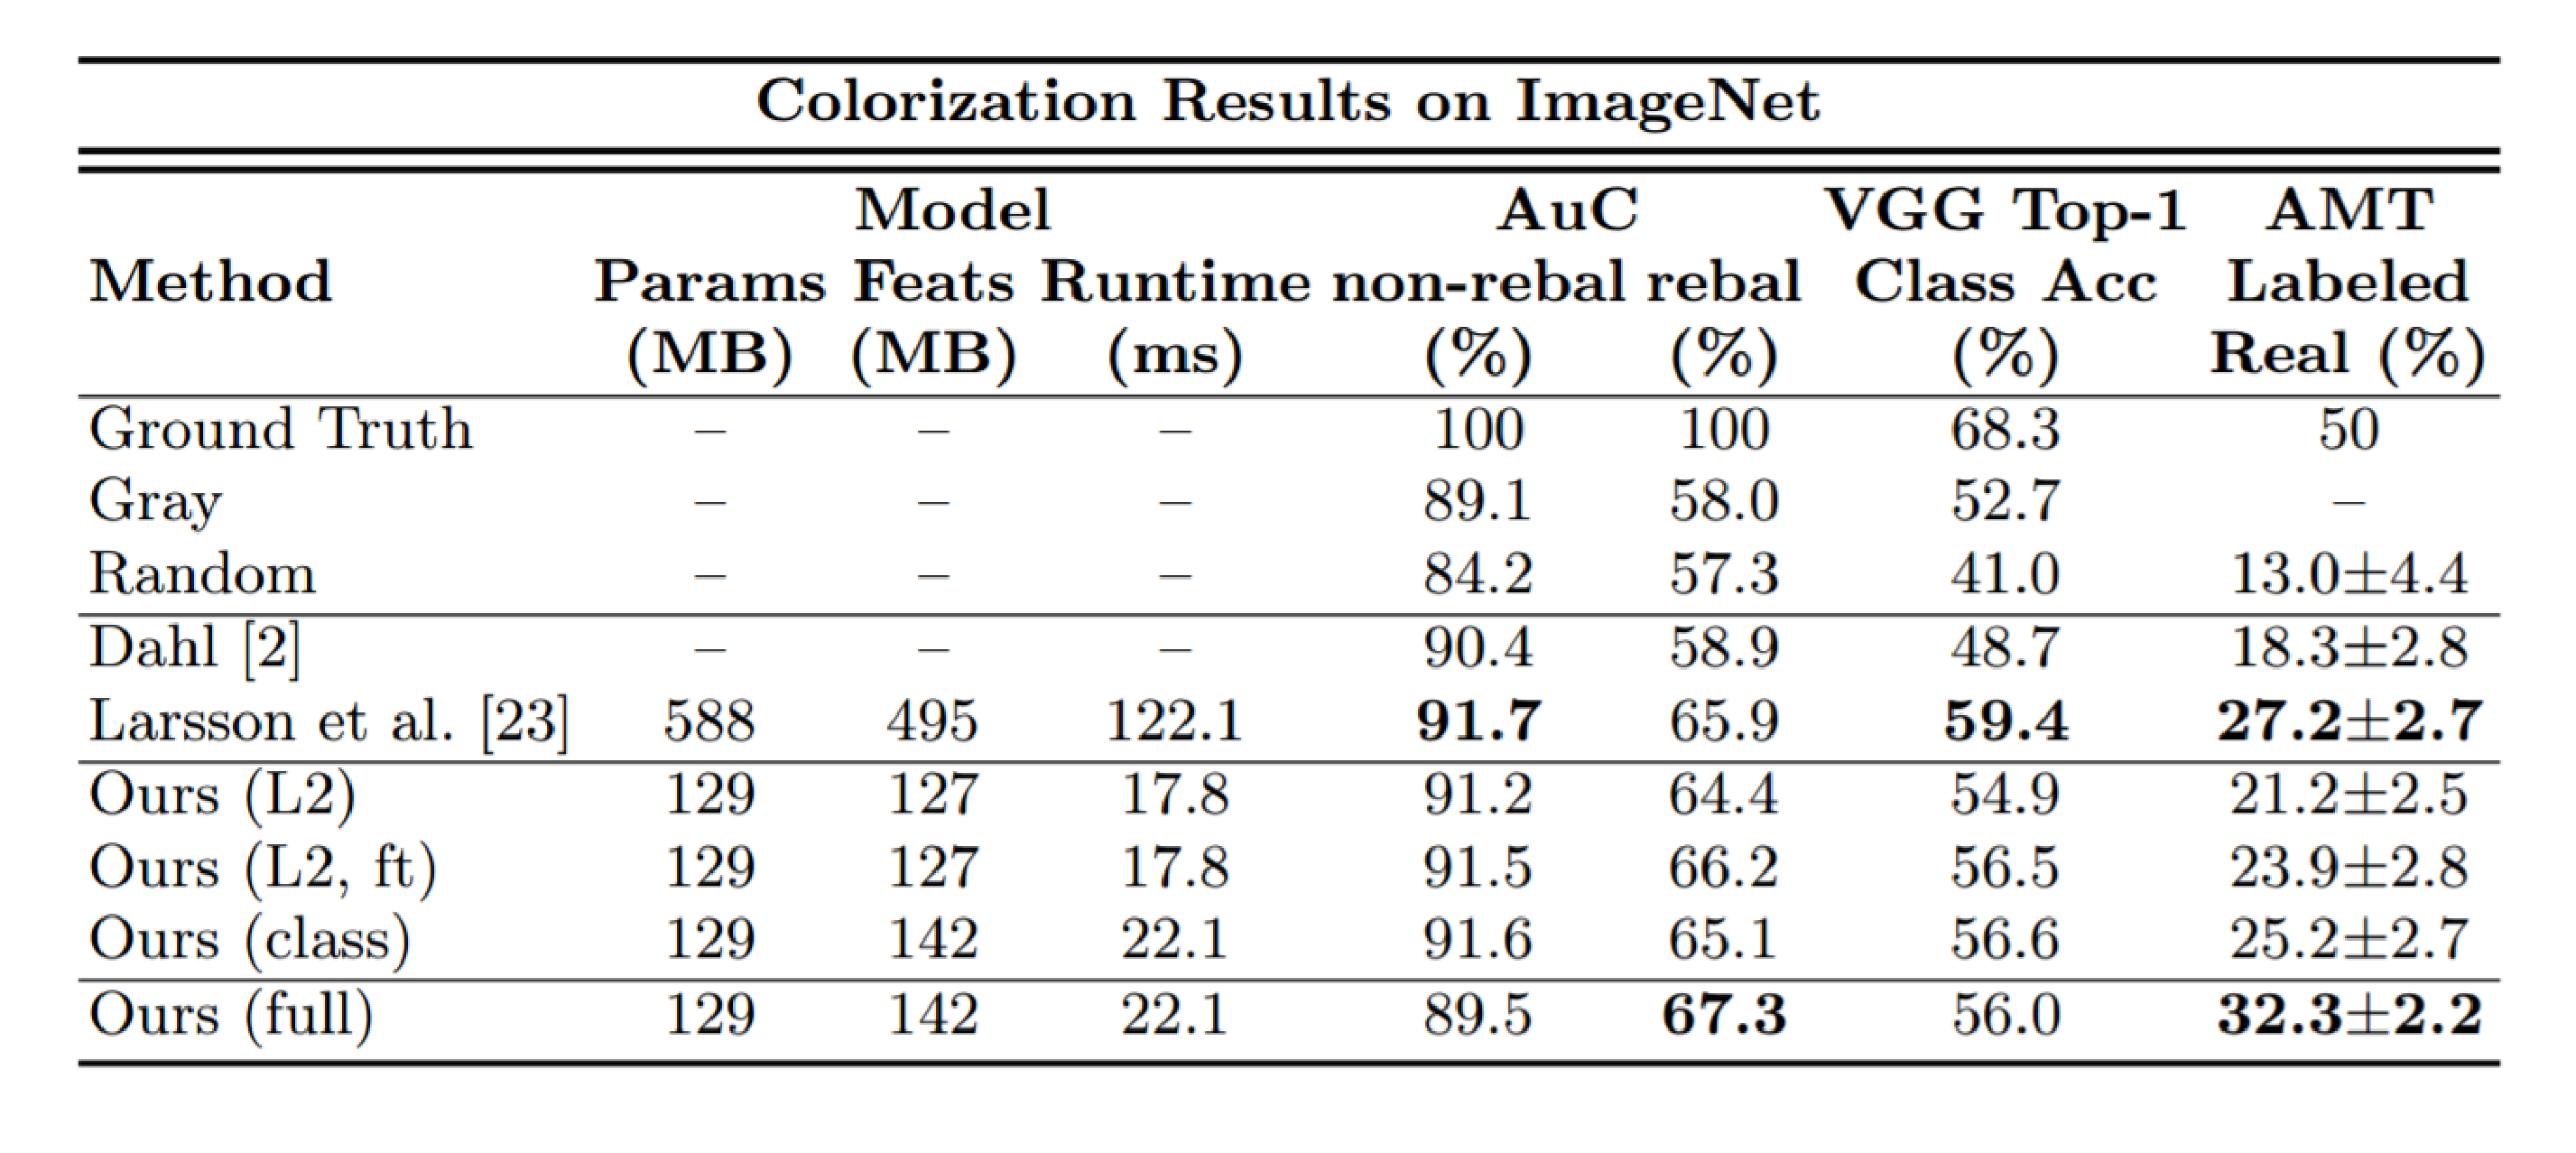
\includegraphics[width=0.7\paperwidth]{appendixT1}
  \caption*{表~1\quad 在ImageNet验证集[28]上10k张图片的着色结果,如[23]。AuC指的是曲线下方累积面积[22]。第二列显示了类别平衡的结果。第三列是在着色后用VGG-16[5]网络分类的准确率。第四列显示了我们在AMT上的真实vs虚假的测试(平均值和标准差都给出了[34])。注意使用两张真实照片期望上会得到50\%的准确率。所有标准都是数值越高越好。每一行表示不同的算法;请看每个算法的文字描述。参数,特征暂用内存以及运行时间在一块Titan X显卡上用Caffe[35]测试}
  \label{tab:badfigure6}
\end{figure}

\subsection{评估着色质量}

我们在ImageNet训练集[28]上的130万图片上训练了我们的网络,用ImageNet验证集上前一万张进行了验证,并且使用了独立于验证集的一万张图片做测试,跟[23]中一样。我们将量化的结果展示在表1中,使用了三种评估方式。一种量化对比对于选择出的成功和失败的例子在图5中可以看到。要看随机图像选择的对比结果,请访问我们的项目网站。


为了特别地测试不同损失函数的效果,我们使用不同的损失训练了我们的CNN。我们也对比了之前[2]与现在的方法[23],它们多使用了在ImageNet上训练的CNN,使用了简单的基准线。

1. \textbf{我们的(完整)} 我们完整的方法,带有公式2中定义的分类损失,和2.2节中定义的类别重新平衡。这个网络用k均值初始化,使用ADAM求解器迭代了大约45万次。

2. \textbf{我们的(分类)} 我们的网络,有分类损失函数,但没有类别重新平衡(公式4中$\lambda = 1$)。

3. \textbf{我们的(L2)} 我们的网络,L2回归损失,如公式1描述,遵照一样的训练参数。

4. \textbf{我们的(L2微调)} 我们的网络,L2回归损失,从我们的完整版本微调而来。

5. \textbf{Larsson等人[23]} 一个CNN的方法,,在之前的处理中也出现过

6. \textbf{Dahl[2]} 一个之前的方法,在VGG特征上使用拉普拉斯金字塔,使用L2回归损失训练

7. \textbf{Gray} 将每个像素上成灰色,即$(a,b)=0$

8. \textbf{随机} 从训练集中随机选一张图片的颜色复制过来。

评估生成图像的质量是一个众所周知的难题,像一些简单的量化评测方法,比如RMS像素颜色差,经常不能抓取视觉真实感。为了解决这些独立评测方法的缺点,我们测试了三种测试不同感觉质量的方法,如表1所示。

1. \textbf{感知真实(AMT): } 对于许多应用,比如图形学中的那些,着色的终极测试就是能否骗过人类观察者。为了测试这一点,我们在AMT(Amazon Mechanical Turk)上进行了一个真实vs虚假的两项强制选择的实验。实验中的参与者被展示了一系列的两张图片。每一对图片包括一张彩色照片和它的重新着色版本,用我们的算法或者其他基准线生成。参与者被要求点击那张他们认为是由计算机程序生成的虚假照片,并且在每一对测试之后,参与者有无限的时间回答。每一个单元测试包含10对练习(不包含到最后分析的结果中),以及40对测试。在练习阶段,参与者会获得他们的选择是否正确的反馈。40对测试时不会给出反馈。每个单元测试只测试一个算法,并且每个参与者被允许最多参与一个单元。总共有40个参与者评估了所有算法。为了确保所有的算法在相同环境下测试(例如,时间,人口统计等等),所有的单元都是同时分发给独立同分布的参与者。

\begin{figure}[h]
  \centering
  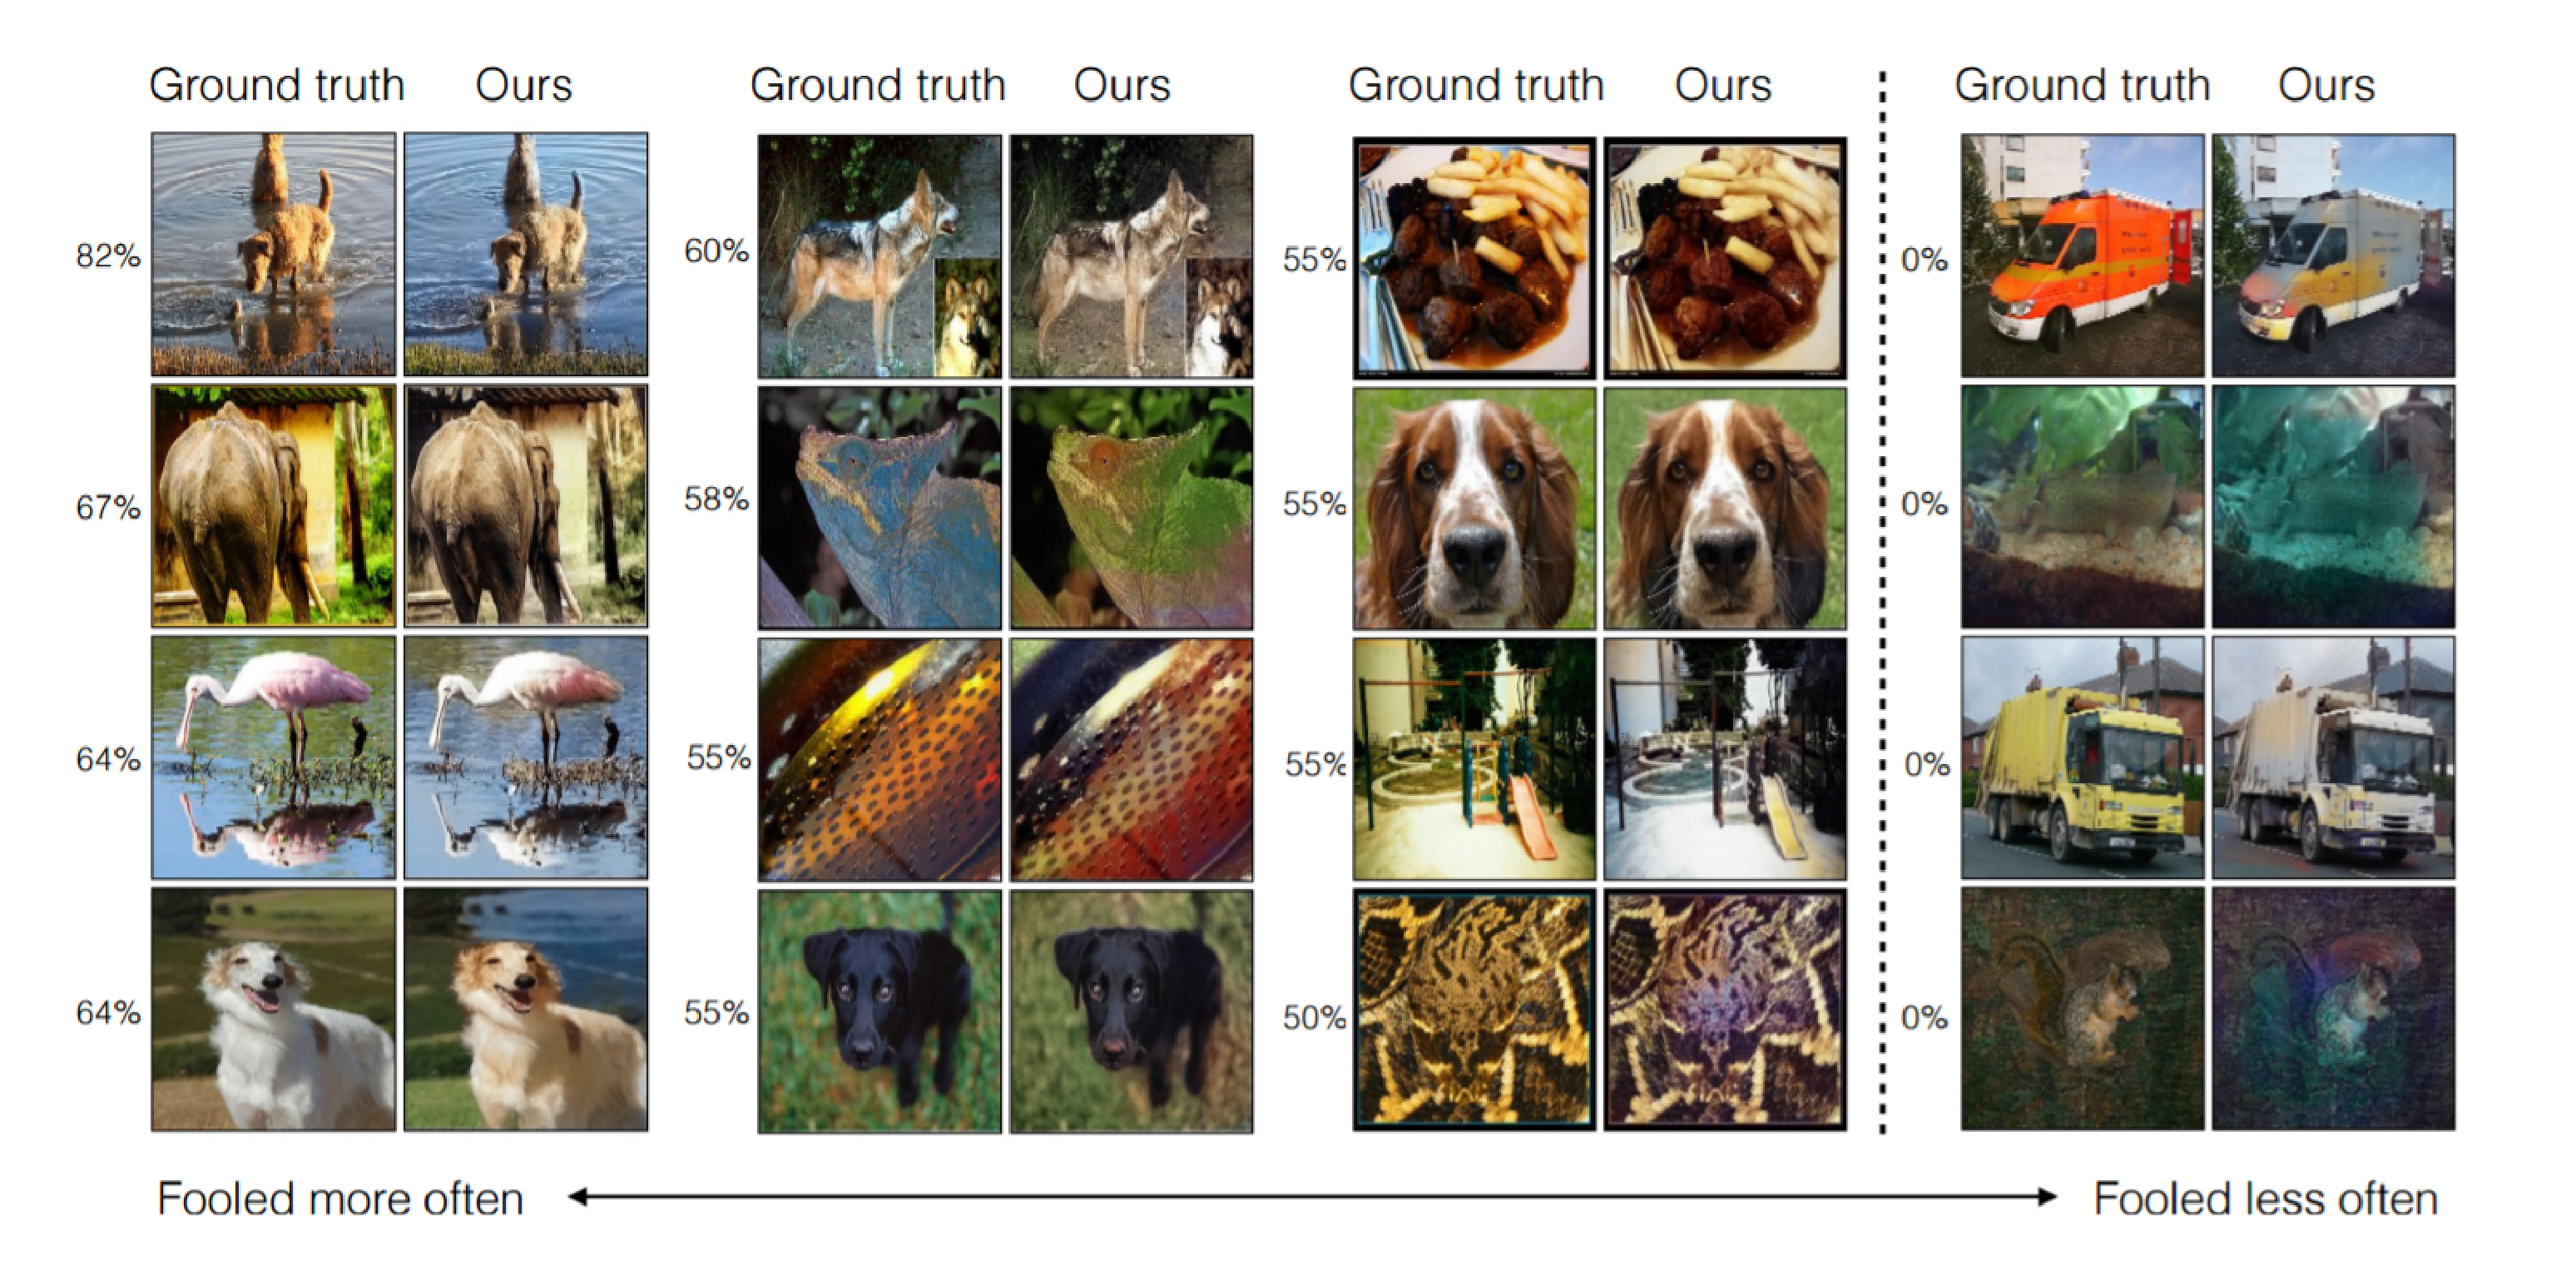
\includegraphics[width=0.7\paperwidth]{appendixF6}
  \caption*{图~6\quad 根据AMT测试者选择我们着色结果而不是真实图片的频率排序的结果。在所有点线左边的图像对,参与者在超过50\%的测试中相信我们的着色比真实图片更真实。在有些例子中,这可能是因为真实图片中糟糕的白平衡,而在被我们的算法修正后,显得更自然。点线的右边是参与者从来没被骗到的例子。}
  \label{tab:badfigure7}
\end{figure}

为了检验参与者在这个任务中是有可信度的,10\%的实验是针对真实照片与随机基准线的。参与者87\%的概率成功的认出了随机着色的图片,证明他们理解了这个任务并且在认真做。

图6给出了参与者在识别我们算法微妙错误的能力的更好的展示。最右一列显示的是那些参与者能100\%成功看出虚假照片的例子。每一对都被至少10个参与者打分。更仔细的观察可以看出在这些图片中,我们的着色算法给出了一些明显的人工痕迹,比如两辆卡车上的黄色斑点,损坏了照片的整体可信度。

但是,我们的完整算法在32\%的测试中欺骗了参与者,如表1所示。这个数字明显比参与比较的其他算法要高(在每个例子中p <0.05),除了Larsson等人的,与他们的差别不明显(p=0.10,所有的数据都由[34]给出)。这些结果验证了使用分类损失和类别重新平衡都是有用的。

注意一点如果我们的算法完全生成了真实照片的结果,在两张一样图片之间的强制选择,会导致参与者被骗的期望概率是50\%。有意思的是,我们有一些例子中参与者有超过50\%的概率被欺骗,表示我们的结果比真实照片更真实。有一些例子在图6的前3列给出。在许多例子中,真实照片的白平衡不好或者有一些不真实的色彩,而我们的系统给出了更实际的表现。

2. \textbf{语义可解释性(VGG分类): } 我们的方法生成的着色结果对于现有的物体识别器是否足够真实呢?我们通过将我们生成的虚假着色图片输入一个被用于ImageNet分类的VGG网络[5]测试了这一点。如果这个分类器表现好,说明我们的着色对物体类别提供了足够准确的信息。使用一个现成的分类器去评测合成数据的真实性在[12]中已经提出来过。

结果显示在表1的右起第二列中。在去除输入图片的颜色后,分类准确率从68.3\%降到了52.7\%。而在用我们的算法重新着色后,准确率提升到了56.0\%(我们方法的其他变种到达了一些稍高的结果)。Larsson等人的方法[23]在这个测试中达到了更好的结果,59.4\%的准确率。作为参考,一个在灰度输入上微调过的VGG分类网络可以达到63.5\%的结果。

除了作为一个感知评估标准,这个分析指出了我们算法的一种实际用处:不需要额外的训练或者微调,我们就能改善灰度图片分类的结果,只要用我们的算法着色然后输入到一个现成的分类器中。

3. \textbf{原始准确率(AuC): } 作为一个低端的测试,我们计算了生成图片像素与真实图片像素ab颜色L2距离在一定阈值内的百分比。然后我们设置阈值从0到150以生成一个累积质量函数,如[22]所说,对曲线(AuC)下的区域求和,并且归一化。注意这个AuC方法测试的是原始预测的准确率,而我们的方法目标是合理性。

我们的网络,分类训练而没有类别重新平衡时,要远好于L2变种(当从头开始训练)。当L2网络从颜色分类网络微调而来,它可以达到分类网络的表现。这表明L2可以达到准确的着色,但是从头开始训练会很难达到最优。Larsson等人[23]的方法达到了稍微好一点的准确率。注意到这个评估方法充满了不饱和的像素,由于ab颜色在自然图像中的分布(图3(b))。结果就是,即使将每个像素预测为灰色也能得到很好的评价,而我们的完整算法也得到类似的分数。

另一方面,图像中的感兴趣的区域倾向于有一个更高饱和度的ab值分布。如此,我们计算了一个类别平衡版本的AuC,通过重新加权像素的颜色概率(公式4,设$\lambda = 0$)。在这样的评估下,我们的完整算法远优于所有变种和其他比较的算法,显示对训练物体做类别重新平衡达到了预计的效果。

\begin{figure}[h]
  \centering
  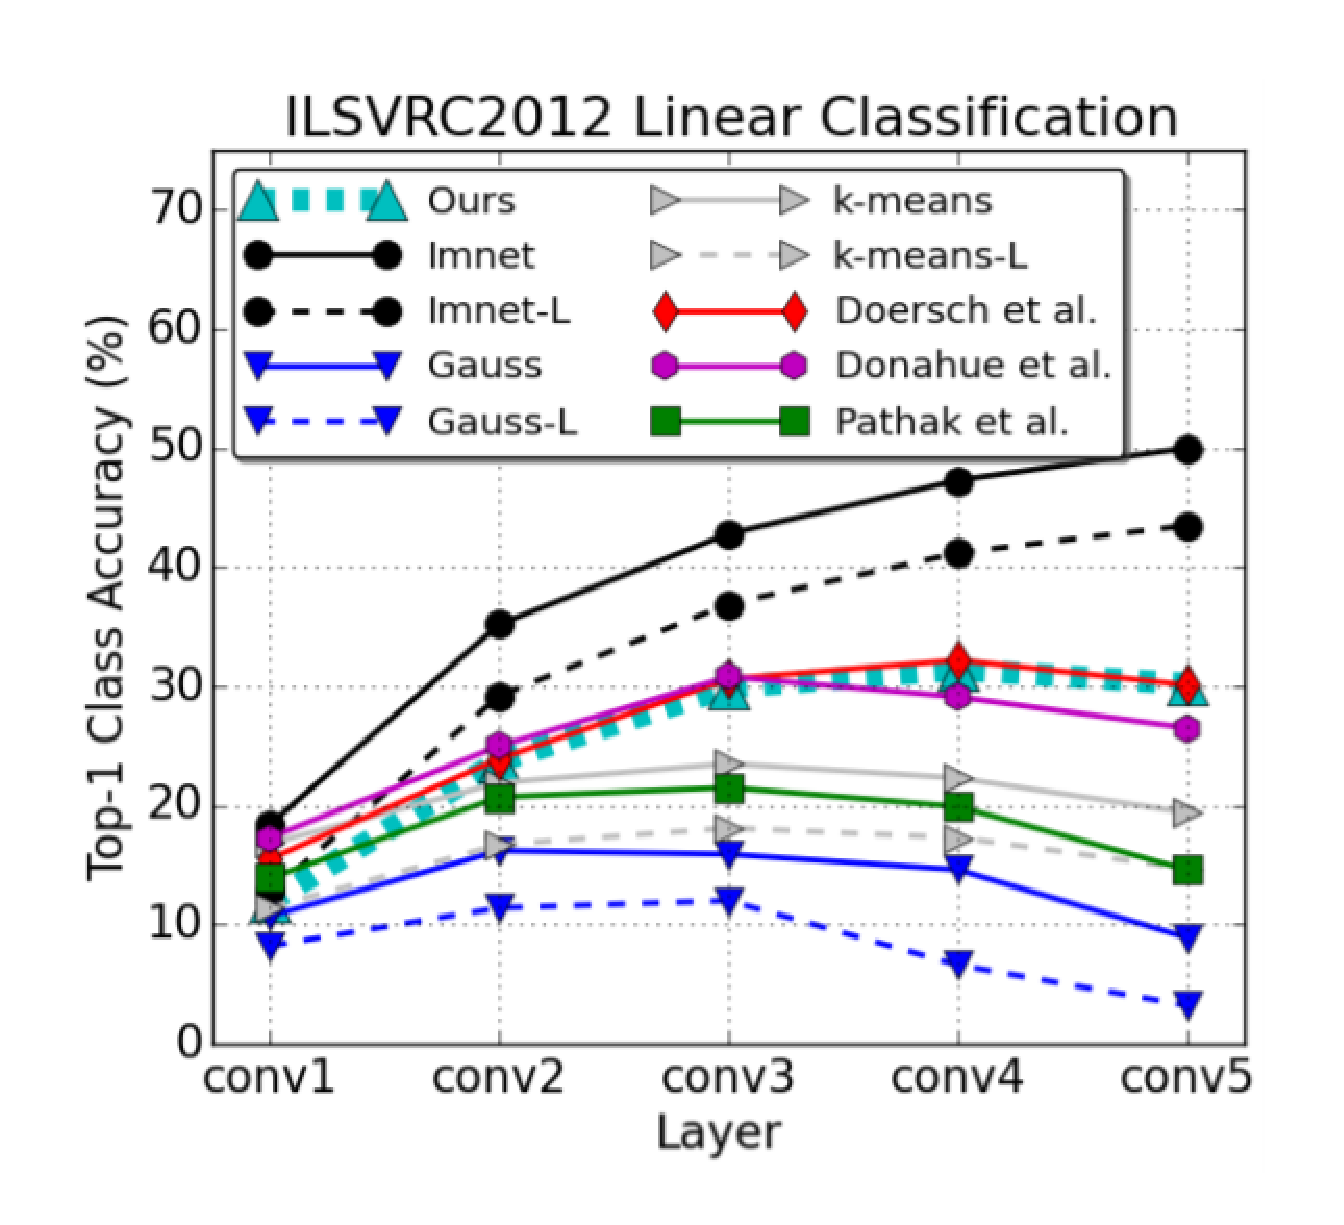
\includegraphics[width=0.7\paperwidth]{appendixF7}
  \caption*{图~7\quad \textbf{ImageNet上的任务综述} 我们固定了预训练的网络并且为ImageNet[28]分类学习了线性分类器。特征被平均池化和相等的核和步幅大小,直到特征维度小于10k。ImageNet[38],k均值[36],以及高斯初始化在灰度输入上运行,用点线表示。彩色输入的结果用连续线给出。之前的[14,10]和现在的[16]工作自监督方法都展示了。}
  \label{tab:badfigure8}
\end{figure}

\begin{figure}[h]
  \centering
  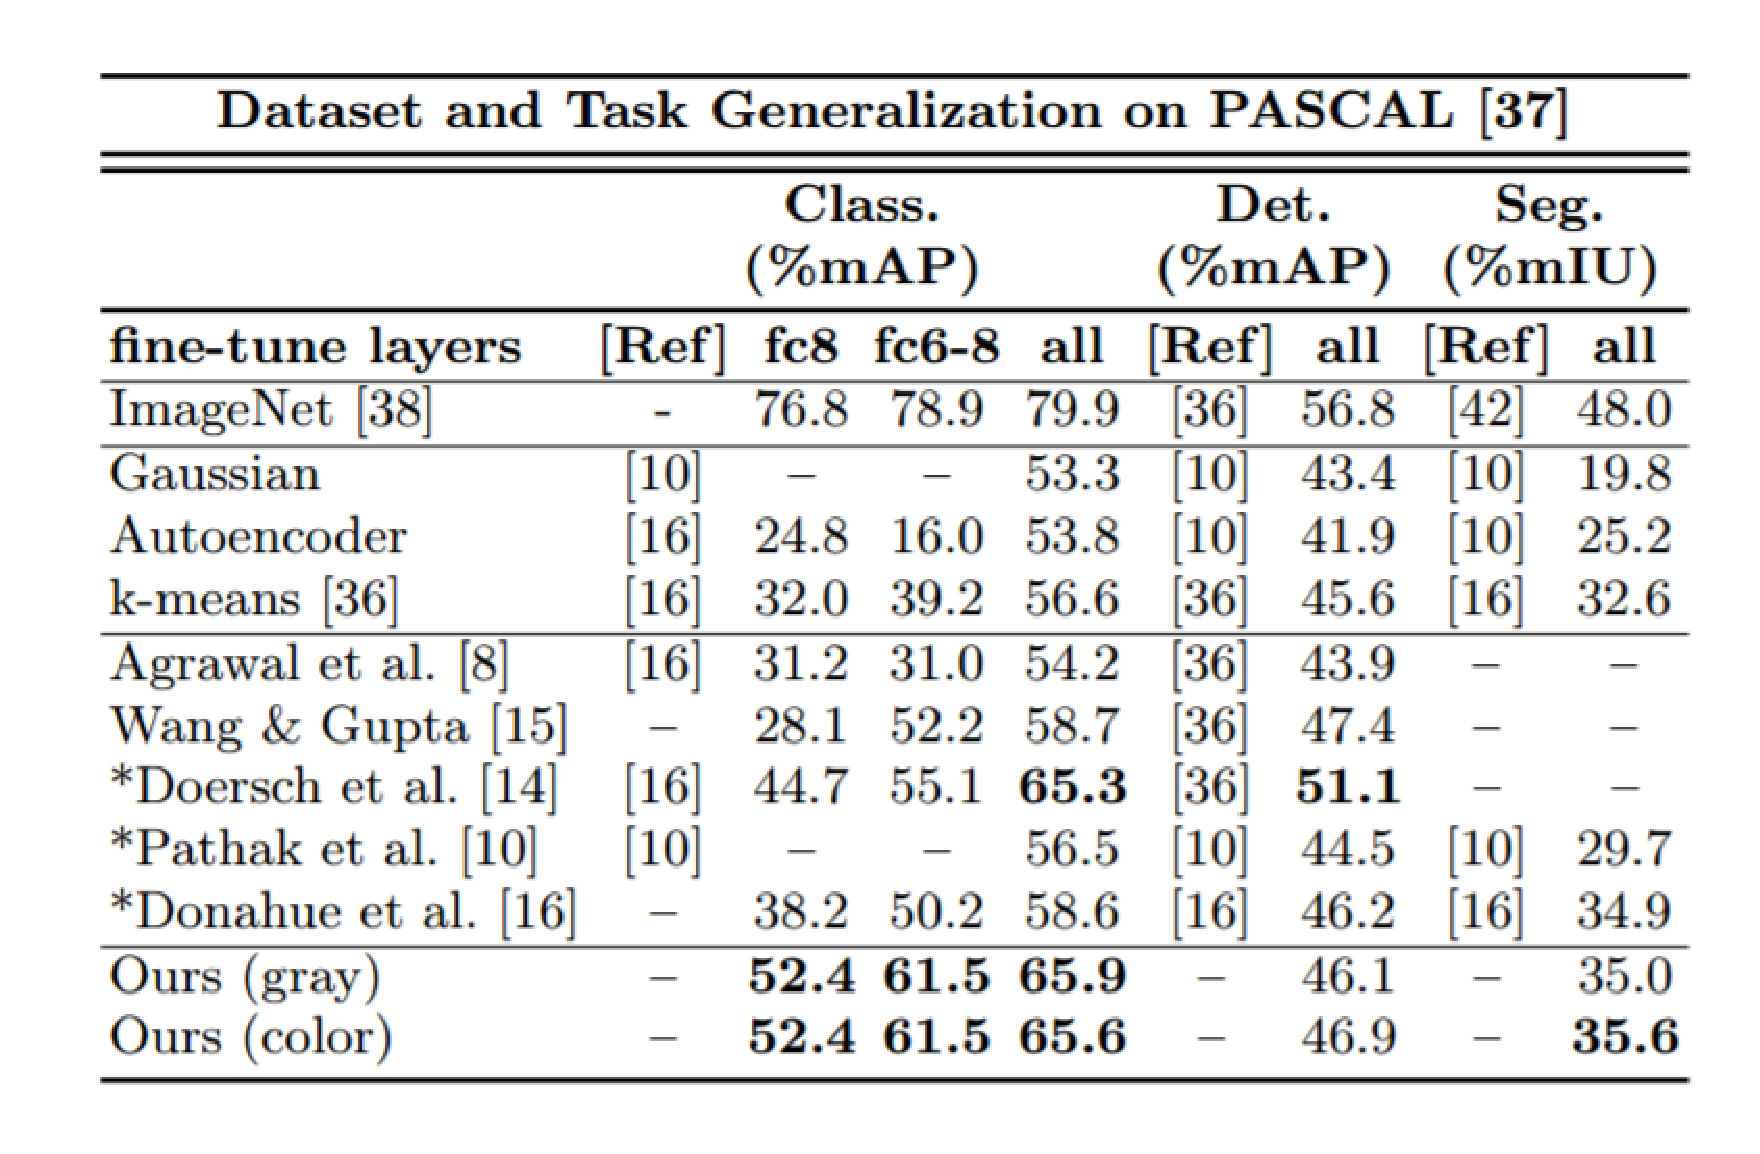
\includegraphics[width=0.7\paperwidth]{appendixT2}
  \caption*{表~2\quad \textbf{PASCAL 上的任务和数据集} PASCAL VOC 2007[39]上的分类和检测任务以及PASCAL VOC 2012[40]上的分割任务,为每个任务使用了标准平均准确率(mAP)和集合平均交集。我们对灰度输入和彩色输入微调了网络。带*的方法只预训练了AlexNet层的子网络。余下的层用[36]初始化。}
  \label{tab:badfigure9}
\end{figure}

\subsection{交叉通道编码作为自监督特征学习}

除了在着色任务上做出了贡献,我们评估了着色如何作为表示学习的前文工作。我们的模型类似于自动编码,除了输入输出是不同的图像通道,于是有术语交叉通道编码。

为了评估通过这种交叉通道编码学习的特征表示,我们在我们的网络上跑了两组测试。首先,我们测试了这个特征的任务泛化能力通过固定学习表示和在已经见过的数据上(图7)训练线性分类器。第二,我们在PASCAL数据集[37]上微调了网络,以适用于分类,检测和分割的任务。在这里,除了在已有的任务测试,这组实验还测试了学习表示的数据泛化能力。为了与之前的特征学习算法公平比较,我们在着色任务上重新训练了一个AlexNet网络[38],使用我们完整的方法迭代了45万次。我们发现结果在物体分类和分割上相比之前的方法达到了更好的表现(表2)。

\textbf{ImageNet分类 } 这个网络是在ImageNet数据集上预训练着色的,没有语义标签的信息。我们测试了学习的特征能多大程度代表物体层面的语义。为了达到这个效果,我们固定了网络参数,提供语义标签,并且在每个卷积层训练线性分类器。结果如图7所示。

在ImageNet分类上直接训练的AlexNet达到了最好的结果,并且为这个测试设立了一个最高标准。随机初始化,用高斯权重或者在[36]中实现的k均值方案,在中间层达到峰值。因为我们的表示是在灰度图片上学习的,在网络的输入上有障碍。为了量化这种信息丢失的影响,我们在灰度图分类上微调了AlexNet,并且采用了随机初始化。有趣的是,对所有三种方法,在彩色和灰度输入之间有6\%的性能差别,这一点在整个网络大致恒定。

我们比较了自己的模型和其他最近在ImageNet上预训练的自监督方法[14,10,16]。	首先,我们的conv1表示相比其他竞争方法[14,16]在线性分类性能上表现更差,但是使用灰度输入时是性能相近的。但是,这个性能差在conv2时立即消失了,我们的网络与其他方法[14,16]整个网络相比达到了同等的性能。这表明尽管有输入障碍,解决着色任务鼓励在训练数据分布中线性的分离语义类别。

\textbf{PASCAL 分类,检测和分割 } 我们在通用的自监督基准PASCAL分类,检测和分割[14,36,10]上测试了我们的模型。结果如表2所示,我们的网络在所有三个任务中都有很强的表现,并且在分类和分割中有最先进的表现。我们使用了[36]的方法,其中调整层的尺度为了让他们能在同样的速率学习。我们在两种模式测试了自己的模型:(1)通过忽略颜色信息保持灰度输入(2)将conv1改成接受3通道Lab输入,初始ab通道的权值为0。

我们首先在PASCAL VOC 2007[39]上测试了网络分类,遵照[16]中的规定。网络通过固定一部分,微调剩下的来训练。注意当conv1固定时,这个网络只能有效的解释灰度图像。在所有的三个分类测试中,我们达到了最好的准确率。

我们同样在PASCAL VOC 2007上测试了检测任务,用快速R-CNN[41],遵照[36]中的流程。Doersch等人[14]达到了51.1\%,而我们使用灰度和彩色输入分别达到了46.9\%和47.9\%。我们的方法远高于强k均值[36]基准线的45.6\%,但是所有的自监督方法依然远落后与在ImageNet上用语义监督预训练的56.8\%的结果。

最后,我们在PASCAL VOC 2012[40]上测试了语义分割,使用[42]的FCN架构,遵照[10]中的规定。我们的着色任务与语义分割任务有相似之处,因为两者都是逐像素的分类问题。我们的灰度微调网络达到了35\%,与Donahue等人[16]的结果相近,添加颜色信息后性能提升到了35.6\%,高于其他测试的算法。

\begin{figure}[h]
  \centering
  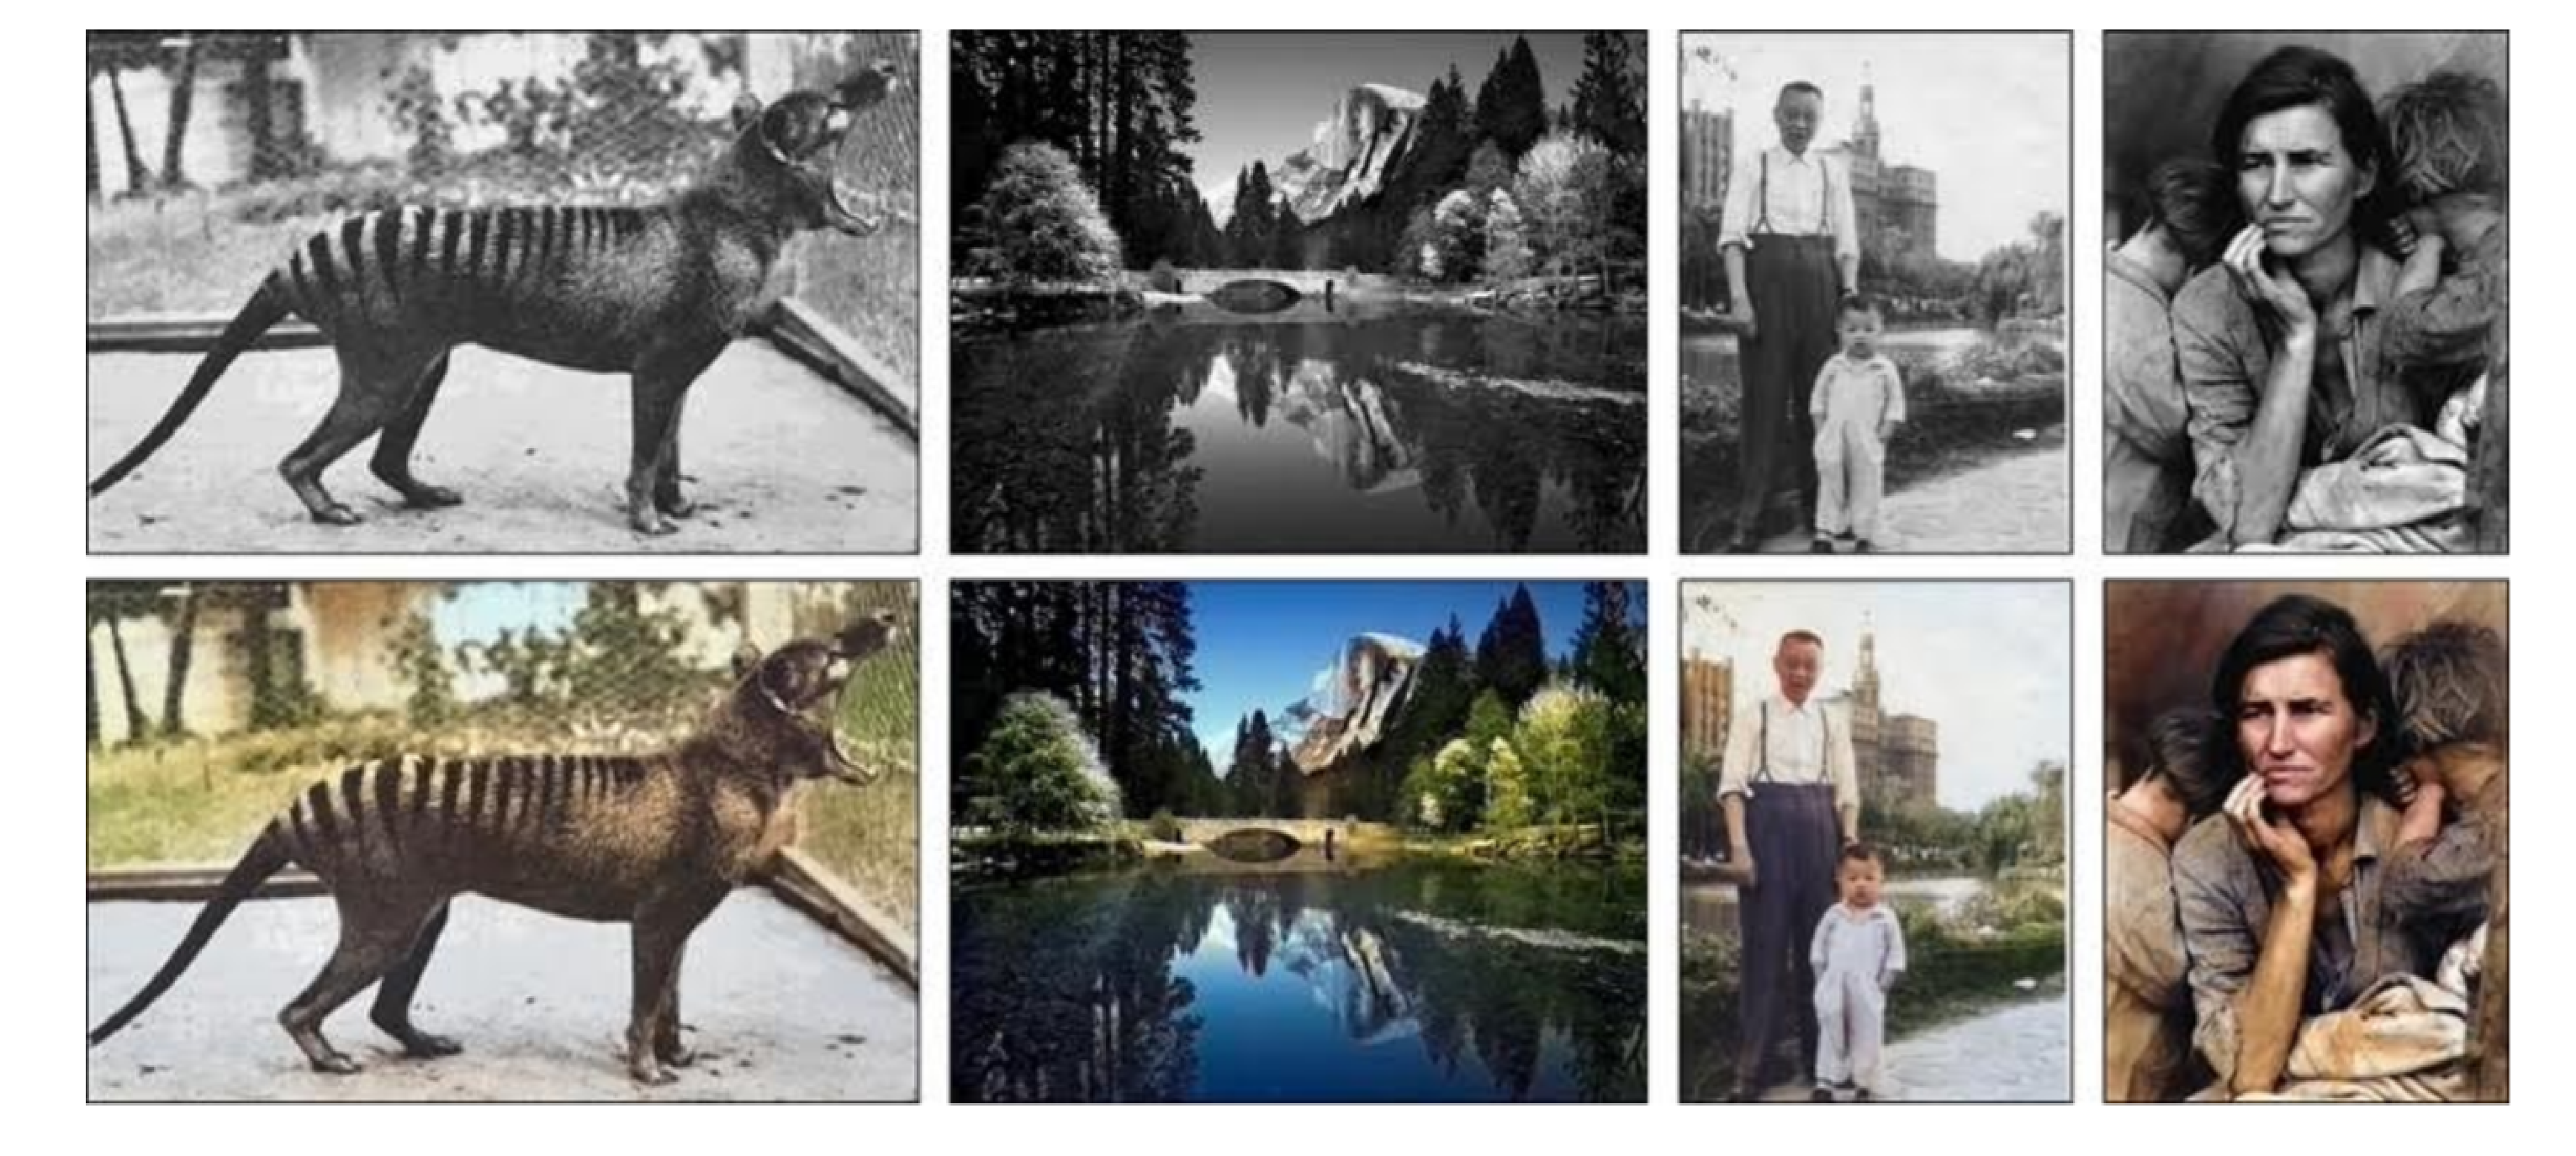
\includegraphics[width=0.7\paperwidth]{appendixF8}
  \caption*{图~8\quad 将我们的算法应用于传统黑白照片。从左到右:David Fleay拍摄的Thylacine,1936;Ansel Adams拍摄的优胜美地;业余爱好者的家庭照,1956;Dorothea Lange的移民母亲,1936}
  \label{tab:badfigure10}
\end{figure}

\subsection{传统黑白老照片}

由于我们的模型是用假的灰度照片训练,因为这些照片是用彩色照片去掉ab通道得到,所以我们也在传统黑白老照片上测试了我们的方法。如图8所示(更多结果可以在我们的项目网页上看到)。可以看出我们的模型依然能够产生良好的着色,尽管照片的低级统计数据与用来训练的现代照片有很大差别。

\section{结论}

虽然图像着色是计算机图形学中的精品任务,它也是计算机视觉中一个困难的像素预测问题。在这里我们展示了使用一个深层CNN与一个精心选择的目标函数能使着色达到与真实照片更近更难区分的结果。我们的方法不仅提供了一个有用的图形学输出,也可以被看成一个表达学习的上游任务。尽管只在颜色上进行了训练,我们的网络也能学习对于物体分类,检测和分割有用的表示,与其他自监督的预训练方法相比有很强的竞争力。

\section*{原文索引}

\begin{translationbib}
\item Cheng, Z., Yang, Q., Sheng, B.: Deep colorization. In: Proceedings of the IEEE International Conference on Computer Vision. (2015) 415–423
\item Dahl, R.: Automatic colorization. In: http://tinyclouds.org/colorize/. (2016)
\item Charpiat, G., Hofmann, M., Sch¨olkopf, B.: Automatic image colorization via multimodalpredictions. In: Computer Vision–ECCV 2008. Springer (2008) 126–139
\item Ramanarayanan, G., Ferwerda, J., Walter, B., Bala, K.: Visual equivalence: towardsa new standard for image fidelity. ACM Transactions on Graphics (TOG)26(3) (2007) 76
\item Simonyan, K., Zisserman, A.: Very deep convolutional networks for large-scaleimage recognition. arXiv preprint arXiv:1409.1556 (2014)
\item Bengio, Y., Courville, A., Vincent, P.: Representation learning: A review and newperspectives. IEEE transactions on pattern analysis and machine intelligence 35(8)(2013) 1798–1828
\item Ngiam, J., Khosla, A., Kim, M., Nam, J., Lee, H., Ng, A.Y.: Multimodal deeplearning. In: Proceedings of the 28th international conference on machine learning(ICML-11). (2011) 689–696
\item Agrawal, P., Carreira, J., Malik, J.: Learning to see by moving. In: Proceedings ofthe IEEE International Conference on Computer Vision. (2015) 37–45
\item Jayaraman, D., Grauman, K.: Learning image representations tied to ego-motion.In: Proceedings of the IEEE International Conference on Computer Vision. (2015)1413–1421
\item Pathak, D., Kr¨ahenb¨uhl, P., Donahue, J., Darrell, T., Efros, A.: Context encoders:Feature learning by inpainting. In: CVPR. (2016)
\item Lotter, W., Kreiman, G., Cox, D.: Deep predictive coding networks for videoprediction and unsupervised learning. arXiv preprint arXiv:1605.08104 (2016)
\item Owens, A., Isola, P., McDermott, J., Torralba, A., Adelson, E.H., Freeman, W.T.:Visually indicated sounds. CVPR (2016)
\item Owens, A., Wu, J., McDermott, J.H., Freeman, W.T., Torralba, A.: Ambient soundprovides supervision for visual learning. In: ECCV. (2016)
\item Doersch, C., Gupta, A., Efros, A.A.: Unsupervised visual representation learningby context prediction. In: Proceedings of the IEEE International Conference onComputer Vision. (2015) 1422–1430
\item Wang, X., Gupta, A.: Unsupervised learning of visual representations using videos.In: Proceedings of the IEEE International Conference on Computer Vision. (2015)2794–28021
\item Donahue, J., Kr¨ahenb¨uhl, P., Darrell, T.: Adversarial feature learning. arXivpreprint arXiv:1605.09782 (2016)1
\item Hertzmann, A., Jacobs, C.E., Oliver, N., Curless, B., Salesin, D.H.: Image analogies.In: Proceedings of the 28th annual conference on Computer graphics andinteractive techniques, ACM (2001) 327–3401
\item Welsh, T., Ashikhmin, M., Mueller, K.: Transferring color to greyscale images.ACM Transactions on Graphics (TOG) 21(3) (2002) 277–2801
\item Gupta, R.K., Chia, A.Y.S., Rajan, D., Ng, E.S., Zhiyong, H.: Image colorizationusing similar images. In: Proceedings of the 20th ACM international conferenceon Multimedia, ACM (2012) 369–378
\item Liu, X., Wan, L., Qu, Y., Wong, T.T., Lin, S., Leung, C.S., Heng, P.A.: Intrinsiccolorization. In: ACM Transactions on Graphics (TOG). Volume 27., ACM (2008)152
\item Chia, A.Y.S., Zhuo, S., Gupta, R.K., Tai, Y.W., Cho, S.Y., Tan, P., Lin, S.: Semanticcolorization with internet images. In: ACM Transactions on Graphics (TOG).Volume 30., ACM (2011) 156
\item Deshpande, A., Rock, J., Forsyth, D.: Learning large-scale automatic image colorization.In: Proceedings of the IEEE International Conference on ComputerVision. (2015) 567–575
\item Larsson, G., Maire, M., Shakhnarovich, G.: Learning representations for automaticcolorization. European Conference on Computer Vision (2016)
\item Iizuka, S., Simo-Serra, E., Ishikawa, H.: Let there be Color!: Joint End-to-endLearning of Global and Local Image Priors for Automatic Image Colorization withSimultaneous Classification. ACM Transactions on Graphics (Proc. of SIGGRAPH2016) 35(4) (2016)
\item Hariharan, B., Arbel´aez, P., Girshick, R., Malik, J.: Hypercolumns for objectsegmentation and fine-grained localization. In: Proceedings of the IEEE Conferenceon Computer Vision and Pattern Recognition. (2015) 447–456
\item Chen, L.C., Papandreou, G., Kokkinos, I., Murphy, K., Yuille, A.L.: Deeplab:Semantic image segmentation with deep convolutional nets, atrous convolution,and fully connected crfs. arXiv preprint arXiv:1606.00915 (2016)
\item Yu, F., Koltun, V.: Multi-scale context aggregation by dilated convolutions. InternationalConference on Learning Representations (2016)
\item Russakovsky, O., Deng, J., Su, H., Krause, J., Satheesh, S., Ma, S., Huang, Z.,Karpathy, A., Khosla, A., Bernstein, M., et al.: Imagenet large scale visual recognitionchallenge. International Journal of Computer Vision 115(3) (2015) 211–252
\item Zhou, B., Lapedriza, A., Xiao, J., Torralba, A., Oliva, A.: Learning deep featuresfor scene recognition using places database. In: Advances in neural informationprocessing systems. (2014) 487–495
\item Ioffe, S., Szegedy, C.: Batch normalization: Accelerating deep network training byreducing internal covariate shift. arXiv preprint arXiv:1502.03167 (2015)
\item Hinton, G., Vinyals, O., Dean, J.: Distilling the knowledge in a neural network.arXiv preprint arXiv:1503.02531 (2015)
\item Farabet, C., Couprie, C., Najman, L., LeCun, Y.: Learning hierarchical featuresfor scene labeling. Pattern Analysis and Machine Intelligence, IEEE Transactionson 35(8) (2013) 1915–1929
\item Kirkpatrick, S., Vecchi, M.P., et al.: Optimization by simmulated annealing. science220(4598) (1983) 671–680
\item Efron, B.: Bootstrap methods: another look at the jackknife. In: Breakthroughsin Statistics. Springer (1992) 569–593
\item Jia, Y., Shelhamer, E., Donahue, J., Karayev, S., Long, J., Girshick, R., Guadarrama,S., Darrell, T.: Caffe: Convolutional architecture for fast feature embedding.In: Proceedings of the 22nd ACM international conference on Multimedia, ACM(2014) 675–678
\item Kr¨ahenb¨uhl, P., Doersch, C., Donahue, J., Darrell, T.: Data-dependent initializationsof convolutional neural networks. International Conference on LearningRepresentations (2016)
\item Everingham, M., Van Gool, L., Williams, C.K., Winn, J., Zisserman, A.: Thepascal visual object classes (voc) challenge. International journal of computervision 88(2) (2010) 303–338
\item Krizhevsky, A., Sutskever, I., Hinton, G.E.: Imagenet classification with deep convolutionalneural networks. In: Advances in neural information processing systems.(2012) 1097–1105
\item Everingham, M., Van Gool, L., Williams, C.K.I., Winn, J., Zisserman, A.:The PASCAL Visual Object Classes Challenge 2007 (VOC2007) Results.http://www.pascal-network.org/challenges/VOC/voc2007/workshop/index.html
\item Everingham, M., Van Gool, L., Williams, C.K.I., Winn, J., Zisserman, A.:The PASCAL Visual Object Classes Challenge 2012 (VOC2012) Results.http://www.pascal-network.org/challenges/VOC/voc2012/workshop/index.html
\item Girshick, R.: Fast r-cnn. In: Proceedings of the IEEE International Conference onComputer Vision. (2015) 1440–1448
\item Long, J., Shelhamer, E., Darrell, T.: Fully convolutional networks for semanticsegmentation. In: Proceedings of the IEEE Conference on Computer Vision andPattern Recognition. (2015) 3431–3440
\item Noroozi, M., Favaro, P.: Unsupervised learning of visual representations by solvingjigsaw puzzles. arXiv preprint arXiv:1603.09246 (2016)
\item Chakrabarti, A.: Color constancy by learning to predict chromaticity from luminance.In: Advances in Neural Information Processing Systems. (2015) 163–171
\item Xiao, J., Hays, J., Ehinger, K.A., Oliva, A., Torralba, A.: Sun database: Large-scalescene recognition from abbey to zoo. In: Computer vision and pattern recognition(CVPR), 2010 IEEE conference on, IEEE (2010) 3485–3492
\item Ratliff, N.D., Silver, D., Bagnell, J.A.: Learning to search: Functional gradienttechniques for imitation learning. Autonomous Robots 27(1) (2009) 25–53
\item Patterson, G., Hays, J.: Sun attribute database: Discovering, annotating, and recognizingscene attributes. In: Computer Vision and Pattern Recognition (CVPR),2012 IEEE Conference on, IEEE (2012) 2751–2758
\end{translationbib}